\documentclass[11pt]{article}
\usepackage[margin=1in]{geometry}
\usepackage{amsmath,amssymb,booktabs,graphicx,hyperref,microtype,xcolor}
\usepackage{tikz}
\usetikzlibrary{arrows.meta,backgrounds,calc,fit,positioning,shapes.geometric}
\newcommand{\squadds}{SQuADDS}
\newcommand{\capop}{CapOp}
\newcommand{\missingfigure}[1]{%
  \fbox{\parbox[c][0.22\textheight][c]{0.91\linewidth}{\centering
  \textbf{Generated panel pending}\\[0.6em]
  Expected file: \texttt{\detokenize{figures/generated/#1}}\\[0.4em]
  This placeholder deliberately makes no empirical claim.}}}
\definecolor{ink}{HTML}{17324D}
\definecolor{teal}{HTML}{1A7F78}
\definecolor{gold}{HTML}{D99B2B}
\definecolor{coral}{HTML}{C95C54}
\definecolor{mist}{HTML}{EDF4F6}
\tikzset{
  flowbox/.style={draw=ink, rounded corners=2pt, very thick, fill=white,
    align=center, inner sep=6pt, font=\small},
  sourcebox/.style={flowbox, fill=coral!8, draw=coral},
  commonbox/.style={flowbox, fill=teal!9, draw=teal},
  resultbox/.style={flowbox, fill=gold!12, draw=gold!90!black},
  flowarrow/.style={-{Stealth[length=2.6mm]}, very thick, draw=ink!75},
  note/.style={font=\scriptsize, text=ink!75, align=center}
}
\title{Physics-aware layout representations for transferable models of planar superconducting devices}
\author{Author list to be finalized}
\date{}

\begin{document}
\maketitle

\begin{abstract}
Electromagnetic simulations for quantum-device design are costly, while the
resulting datasets remain fragmented across component generators, parameter
dictionaries, and design tools. We develop a deterministic representation that
maps planar GDS geometry, ground, conductor connectivity, and arbitrary terminal
sets into a common physics-aware space. We first evaluate the representation
itself: nuisance invariance, sensitivity and smoothness under physical changes,
feature-block contributions, component-family structure, and preservation of
galvanic topology. We then test whether representation distance carries
capacitance information, whether a shared model improves on native tabular
baselines, and whether source-family training reduces the target simulations
needed for unseen families and composite multi-terminal systems.
The arbitrary-terminal v4 views passed all nine frozen planar numerical gates.
Across three families, their mean within-family $R^2$ values in
$\log(1+C)$ were 0.987, 0.986, and 0.978. Representation distance was only
modestly associated with capacitance difference ($\rho=0.251$), and historical
cross-family transfer did not consistently outperform target-only fitting.
Training-family diversity nevertheless improved a matched-budget generalist,
while a three-terminal composite established structural---but not yet
high-fidelity predictive---zero-shot generalization.
The planar interface is designed to accept a future material-stack sidecar, but
multi-plane and flip-chip generalization are outside the present validation
scope.
\end{abstract}

\section*{Introduction}
High-fidelity electromagnetic simulation is a bottleneck in superconducting
quantum-hardware design. Individual groups amortize this cost through parameter
sweeps, interpolation, and surrogate models, but each table is normally tied to
one component generator. A parameter such as \texttt{finger\_length} in an
interdigital capacitor has no literal counterpart in a transverse-cross device,
even when both layouts pose related electrostatic questions. The incompatibility
becomes most costly when a new topology requires another large simulation
campaign.

\begin{figure}[t]
\centering
\resizebox{\textwidth}{!}{%
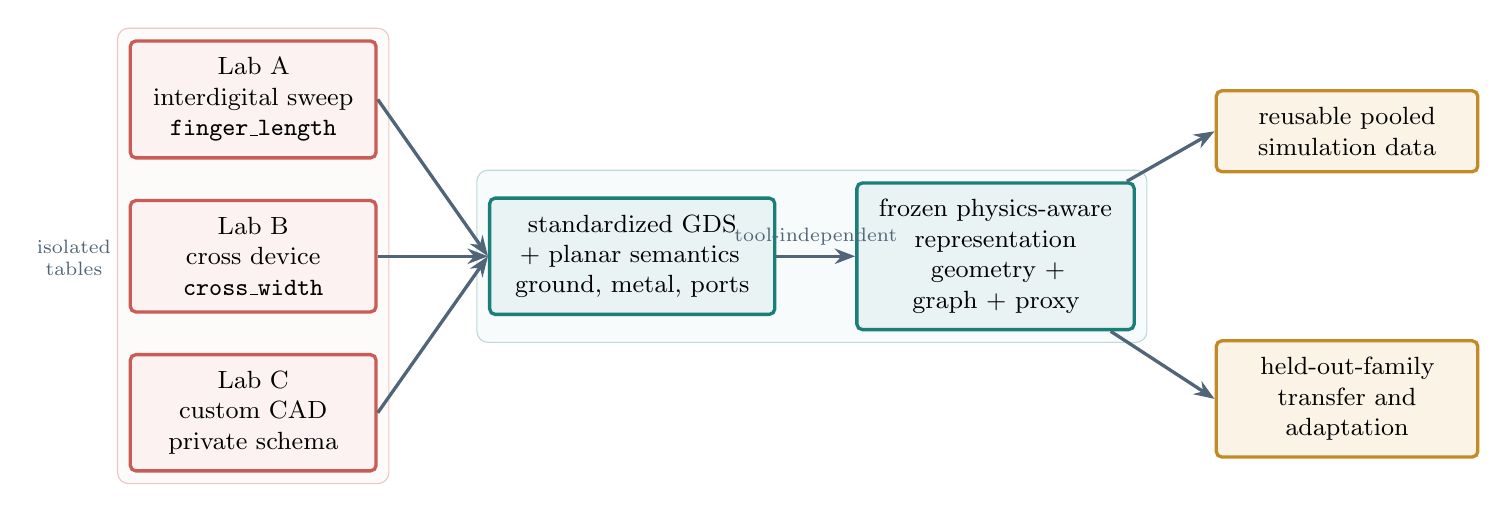
\begin{tikzpicture}[node distance=5mm and 10mm]
  \node[sourcebox, text width=27mm] (a) {Lab A\\interdigital sweep\\\texttt{finger\_length}};
  \node[sourcebox, text width=27mm, below=of a] (b) {Lab B\\cross device\\\texttt{cross\_width}};
  \node[sourcebox, text width=27mm, below=of b] (c) {Lab C\\custom CAD\\private schema};
  \node[note, left=1mm of b, anchor=e] (frag) {isolated\\tables};
  \node[commonbox, text width=32mm, right=14mm of b] (gds) {standardized GDS\\+ planar semantics\\ground, metal, ports};
  \node[commonbox, text width=31mm, right=of gds] (embed) {frozen physics-aware\\representation\\geometry + graph + proxy};
  \node[resultbox, text width=29mm, above right=1mm and 10mm of embed] (reuse) {reusable pooled\\simulation data};
  \node[resultbox, text width=29mm, below right=1mm and 10mm of embed] (tasks) {held-out-family\\transfer and adaptation};
  \draw[flowarrow] (a.east) -- (gds.west);
  \draw[flowarrow] (b.east) -- (gds.west);
  \draw[flowarrow] (c.east) -- (gds.west);
  \draw[flowarrow] (gds) -- node[note, above]{tool-independent} (embed);
  \draw[flowarrow] (embed) -- (reuse.west);
  \draw[flowarrow] (embed) -- (tasks.west);
  \begin{scope}[on background layer]
    \node[fit=(a)(b)(c), fill=coral!3, draw=coral!35, rounded corners=4pt,
      inner sep=4pt] {};
    \node[fit=(gds)(embed), fill=teal!3, draw=teal!30, rounded corners=4pt,
      inner sep=4pt] {};
  \end{scope}
\end{tikzpicture}}
\caption{From fragmented tables to a shared layout interface. Native parameter
dictionaries remain useful within a generator but do not define common features
across families. Standardized planar GDS and explicit semantics provide the
input to one frozen representation. The downstream reuse and transfer arrows
state the hypotheses tested in this paper; they are not assumed consequences of
the file format.}
\label{fig:fragmentation}
\end{figure}

GDS is a more portable interface than the code that generated a component, but
geometry alone is not yet a scientific representation. A useful encoder must
distinguish physical scale from drawing pose, identify ground and galvanically
connected conductors, preserve terminal identity without depending on arbitrary
terminal ordering, and expose the correct structure of a variable-size
capacitance matrix. It should detect physically important changes at both small
and large scales without responding strongly to irrelevant translations or
rotations.

Here we ask three questions. First, can a static planar GDS embedding satisfy a
predeclared physical and topological contract across heterogeneous Qiskit Metal
and \squadds{} components? Second, does the resulting geometry carry enough
capacitance information to outperform family-specific tabular representations
and predict which families can transfer useful knowledge? Third, can a
generalist representation recognize a newly composed multi-terminal system and
adapt with a small number of new simulations? We treat all three as empirical
questions and separate representation acceptance from downstream accuracy.

\section*{Results}

\subsection*{A static planar representation with an explicit physical contract}
The encoder begins with a planar GDS semantics contract for signal metal,
ground, terminals, and connectivity. Polygon processing produces connected
conductor bodies and their relationships to local ground. Geometry, physical
scale, proximity, topology, and a deterministic low-fidelity capacitance proxy
are recorded as identifiable feature blocks. The multi-terminal interface
represents an arbitrary conductor/terminal set and supports a matrix-valued
capacitance target rather than reducing every device to one ordered terminal
pair.

Translation, in-plane rotation, reflection, and irrelevant outer-domain crop
are treated as nuisance transformations. Uniform scale, gap, overlap, width,
facing length, ground clearance, body count, terminal configuration, and
galvanic joins are physical transformations. These assignments are frozen
before aggregate scores are calculated.

\begin{figure}[t]
\centering
\resizebox{\textwidth}{!}{%
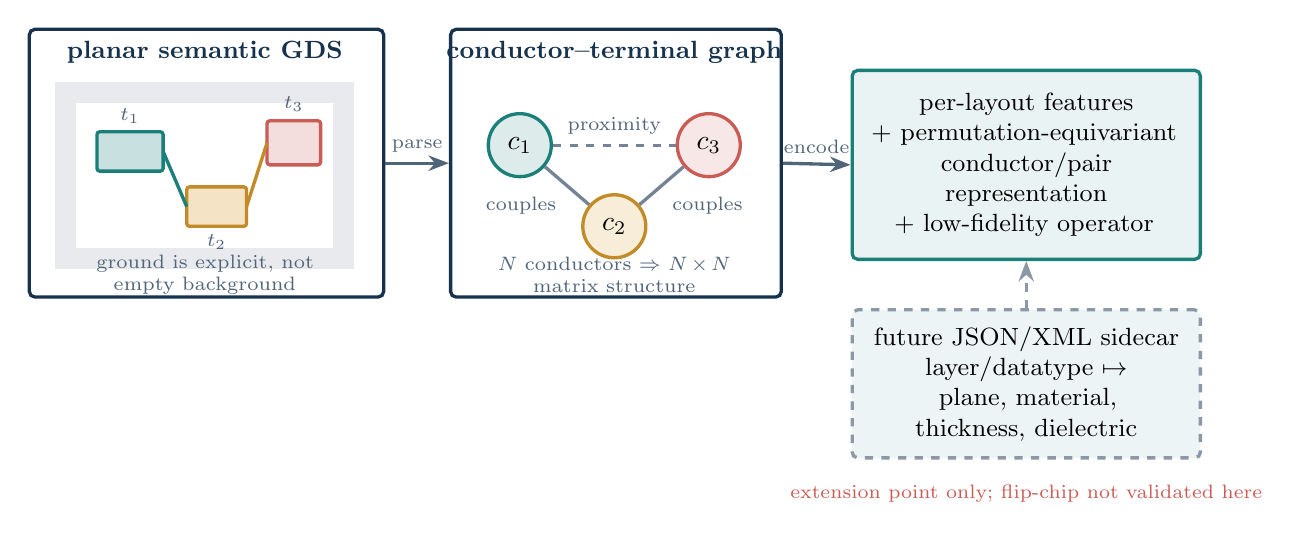
\begin{tikzpicture}[x=1cm,y=1cm]
  % Layout panel
  \node[flowbox, minimum width=4.5cm, minimum height=3.4cm, anchor=south west]
    (layoutframe) at (0,0) {};
  \node[font=\bfseries\small, text=ink] at (2.25,3.13) {planar semantic GDS};
  \fill[ink!10] (0.35,0.38) rectangle (4.15,2.75);
  \fill[white] (0.62,0.65) rectangle (3.88,2.48);
  \draw[very thick, teal, fill=teal!24, rounded corners=1pt]
    (0.88,1.62) rectangle (1.72,2.12);
  \draw[very thick, gold!90!black, fill=gold!28, rounded corners=1pt]
    (2.02,0.92) rectangle (2.78,1.42);
  \draw[very thick, coral, fill=coral!20, rounded corners=1pt]
    (3.04,1.70) rectangle (3.72,2.26);
  \draw[very thick, teal] (1.72,1.87) -- (2.02,1.17);
  \draw[very thick, gold!90!black] (2.78,1.17) -- (3.04,1.98);
  \node[note] at (1.30,2.32) {$t_1$};
  \node[note] at (2.40,0.72) {$t_2$};
  \node[note] at (3.38,2.47) {$t_3$};
  \node[note, text width=3.7cm] at (2.25,0.30)
    {ground is explicit, not empty background};

  % Graph panel
  \node[flowbox, minimum width=4.2cm, minimum height=3.4cm, anchor=south west]
    (graphframe) at (5.35,0) {};
  \node[font=\bfseries\small, text=ink] at (7.45,3.13) {conductor--terminal graph};
  \node[circle, draw=teal, very thick, fill=teal!15, minimum size=8mm] (g1) at (6.25,1.95) {$c_1$};
  \node[circle, draw=gold!90!black, very thick, fill=gold!18, minimum size=8mm] (g2) at (7.45,0.92) {$c_2$};
  \node[circle, draw=coral, very thick, fill=coral!14, minimum size=8mm] (g3) at (8.65,1.95) {$c_3$};
  \draw[very thick, ink!60] (g1) -- node[note, below left]{couples} (g2);
  \draw[very thick, ink!60] (g2) -- node[note, below right]{couples} (g3);
  \draw[very thick, ink!60, dashed] (g1) -- node[note, above]{proximity} (g3);
  \node[note, text width=3.7cm] at (7.45,0.30)
    {$N$ conductors $\Rightarrow$ $N\!\times\!N$ matrix structure};

  % Embedding panel
  \node[commonbox, text width=4.0cm, minimum height=2.4cm, anchor=west]
    (rep) at (10.45,1.70) {per-layout features\\+ permutation-equivariant\\conductor/pair representation\\+ low-fidelity operator};
  \draw[flowarrow] (layoutframe.east) -- node[note, above]{parse} (graphframe.west);
  \draw[flowarrow] (graphframe.east) -- node[note, above]{encode} (rep.west);

  % Future sidecar contract
  \node[flowbox, dashed, draw=ink!50, fill=mist, text width=4.0cm,
    anchor=north west] (sidecar) at (10.45,-0.12)
    {future JSON/XML sidecar\\layer/datatype $\mapsto$ plane, material,
    thickness, dielectric};
  \draw[flowarrow, dashed, draw=ink!50] (sidecar.north) -- (rep.south);
  \node[note, text=coral, below=2mm of sidecar]
    {extension point only; flip-chip not validated here};
\end{tikzpicture}}
\caption{Planar arbitrary-terminal and future stack contract. The planar GDS
parser identifies ground, connected conductor bodies, and attached terminals;
the graph determines the matrix structure and must transform equivariantly when
terminal labels are permuted. A versioned material-stack sidecar is reserved as
an additive input for later multi-plane work. No stack-awareness result is
claimed in the present planar study.}
\label{fig:contract}
\end{figure}

In the first frozen planar acceptance run, the v4 layout, graph-pair, and
hybrid-pair views each passed all nine numerical gates; the v2 and conditioned
v2 controls passed five of nine. At an arbitrary $37^\circ$ rotation, relative
drift was $9\times10^{-6}$ for the v4 layout view, $1\times10^{-5}$ for the
graph-pair view, and $8.06\times10^{-4}$ for the hybrid view, all below the
predeclared $3\times10^{-3}$ threshold. These are numerical tests on controlled
GDS counterfactuals, not evidence for multi-plane invariance.

The v4 layout view pools a 64-coordinate global block, three 64-coordinate
statistics of conductor-node features, and three 96-coordinate statistics of
pair-edge features. The reciprocal graph-pair view concatenates global,
endpoint-sum, endpoint-difference, selected-edge, and all-other-conductor
context blocks. The production hybrid pair view combines the 240-coordinate v3
fixed-stack pair core with 192 coordinates of all-other-conductor context.

\begin{figure}[t]
\centering
\IfFileExists{figures/generated/acceptance_scorecard.png}{%
  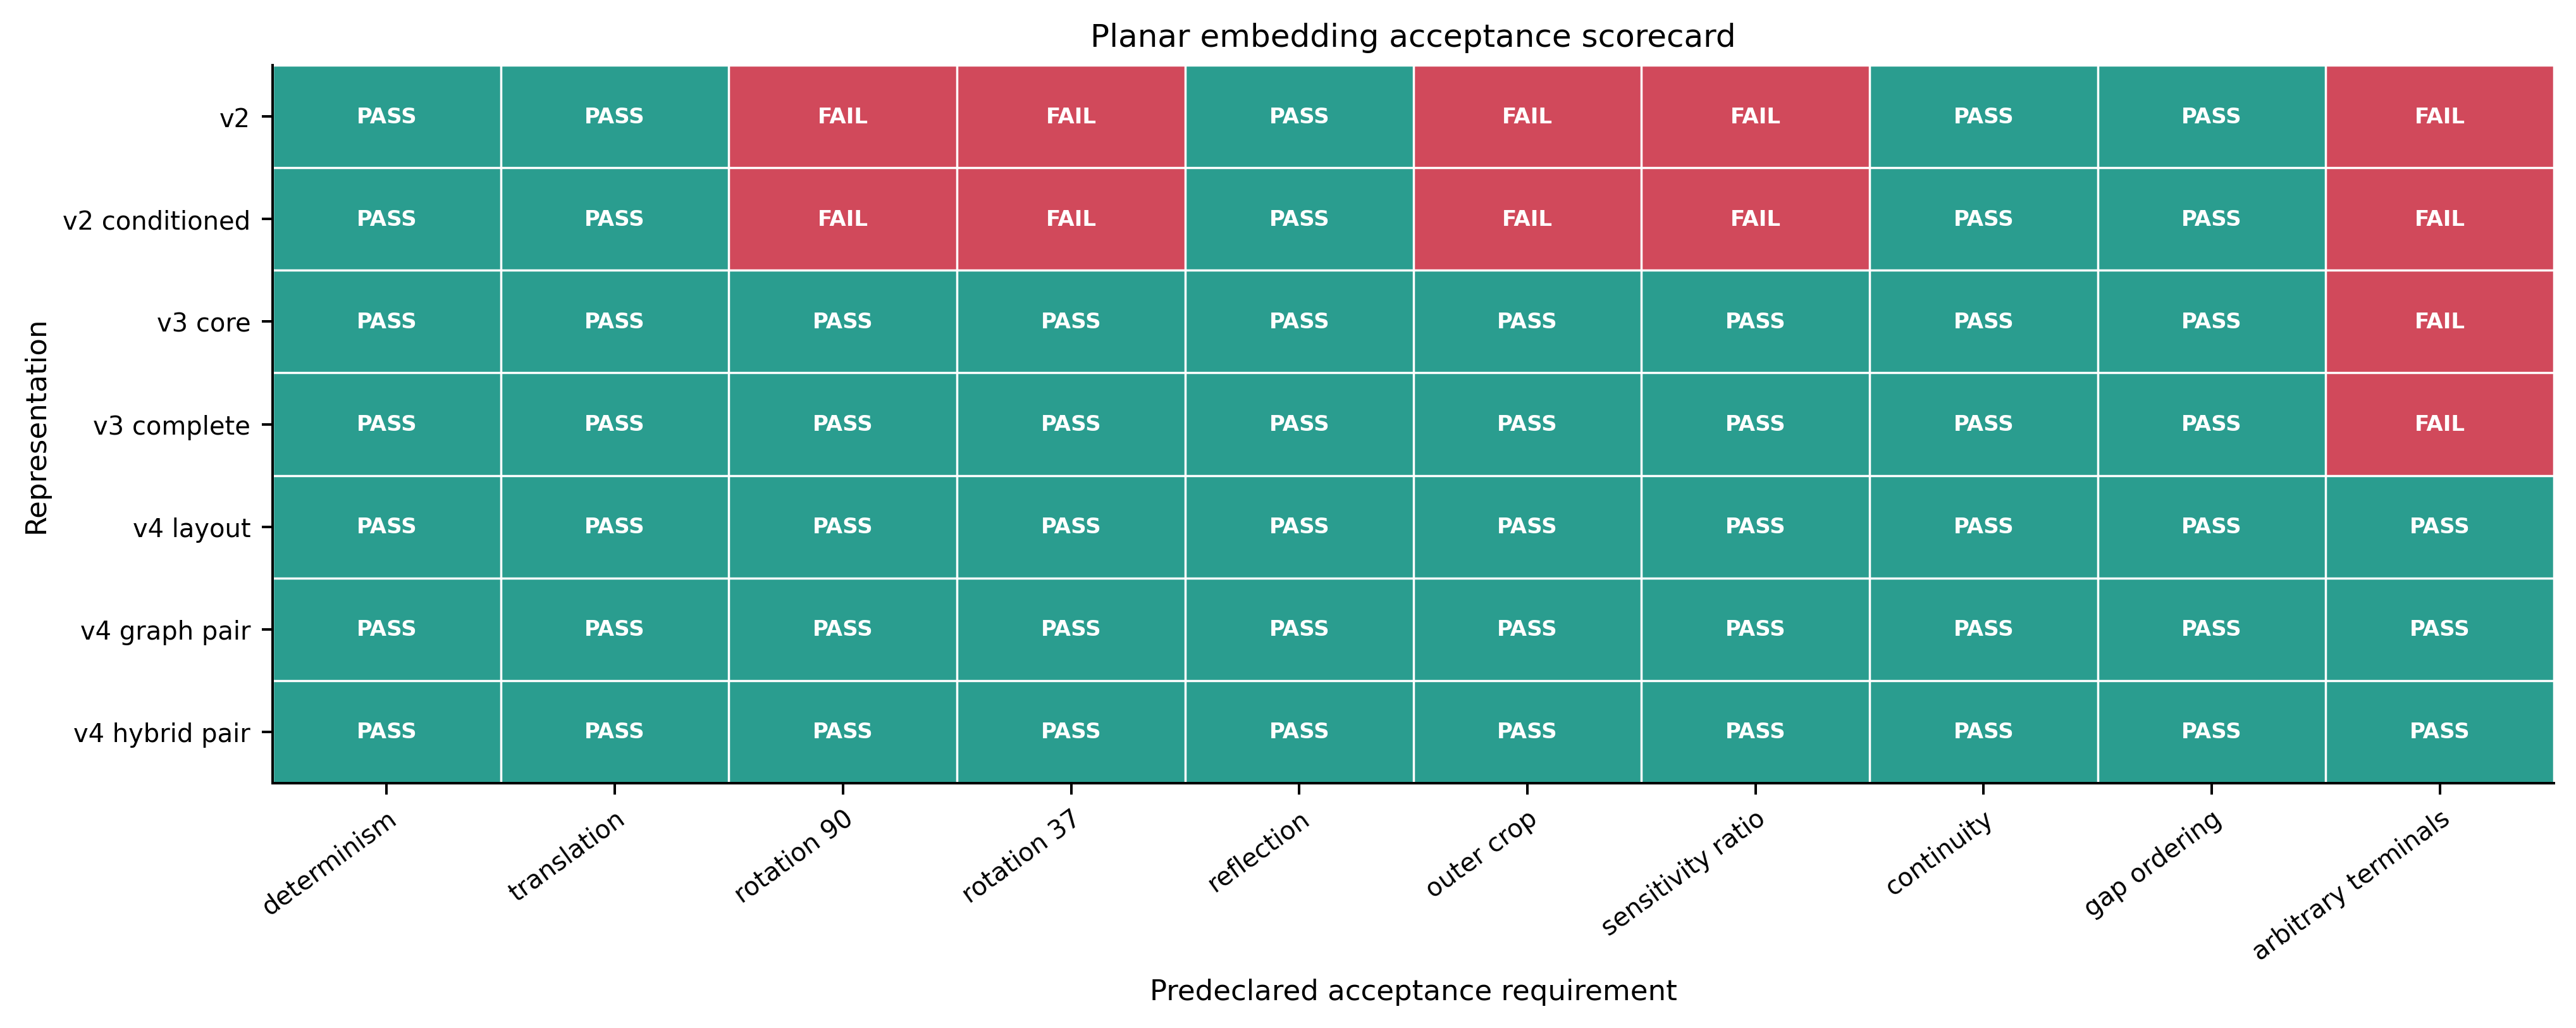
\includegraphics[width=\linewidth]{figures/generated/acceptance_scorecard.png}%
}{\missingfigure{acceptance_scorecard.png}}
\caption{Frozen planar representation acceptance scorecard. The text reports
the established nine-gate totals and arbitrary-rotation drift values. This
panel exposes each gate and representation view separately so an aggregate
pass count cannot hide a failed physical contract.}
\label{fig:acceptance-scorecard}
\end{figure}

\subsection*{Small and large physical changes produce detectable, smooth signals}
We generate paired narrow- and broad-range sweeps over representative physical
parameters. For each path we measure full-vector displacement, block-level
displacement, local finite differences, and discontinuities near any histogram
or basis boundaries. Pose controls are run on the same layouts. Cumulative and
drop-one-block ablations compare v2 and later candidates and identify whether
each block contributes desired sensitivity rather than nuisance leakage.

All v4 views responded smoothly to the four controlled paths and preserved
perfect rank ordering along the terminal-gap path. In the layout-view
cumulative and drop-one ablations, the physical-to-nuisance response ratio
remained between $9.4\times10^3$ and $1.13\times10^4$, so no single retained
pooled block was solely responsible for the invariance result.

\begin{figure}[t]
\centering
\IfFileExists{figures/generated/physical_trajectories.png}{%
  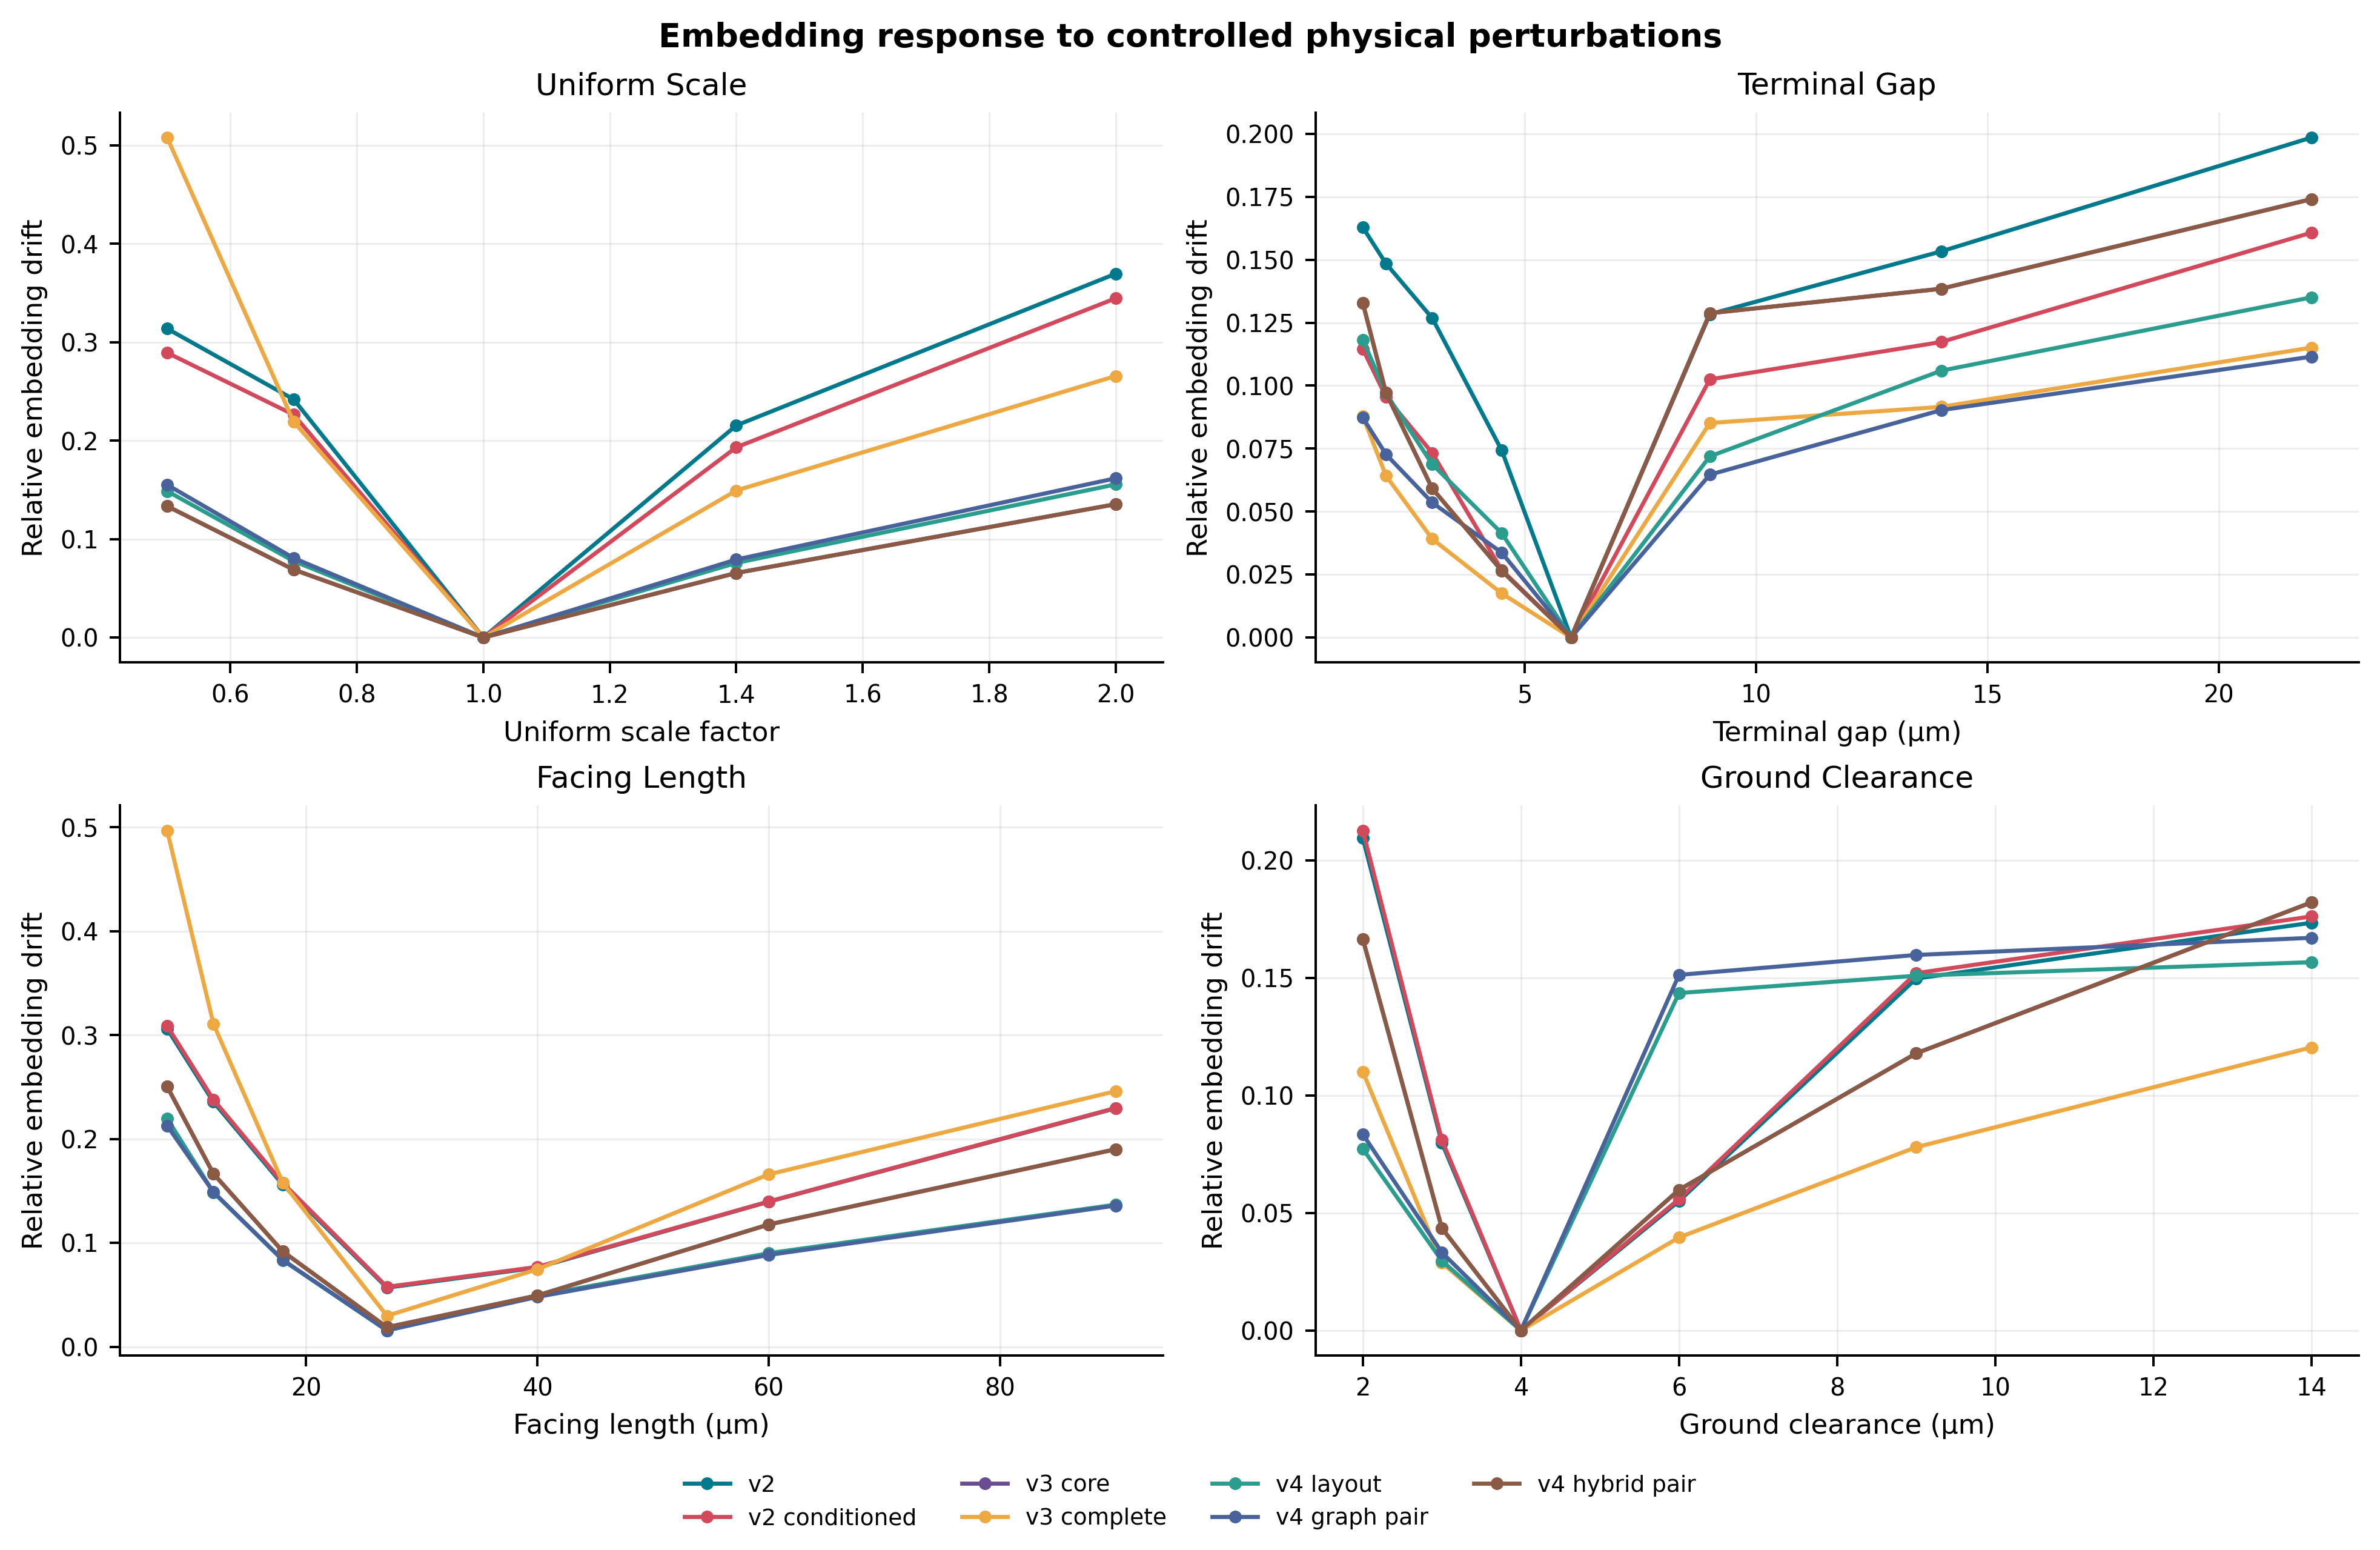
\includegraphics[width=\linewidth]{figures/generated/physical_trajectories.png}%
}{\missingfigure{physical_trajectories.png}}
\caption{Controlled physical trajectories at narrow and broad scales. The
panels compare parameter change with full-vector displacement. The v4 views
leave the baseline smoothly for uniform scale, terminal gap, facing length,
and local ground clearance while maintaining the frozen continuity and
gap-ordering gates. Monotonicity is interpreted only where a physical direction
was declared in advance.}
\label{fig:physical-trajectories}
\end{figure}

\begin{figure}[t]
\centering
\IfFileExists{figures/generated/block_ablation.png}{%
  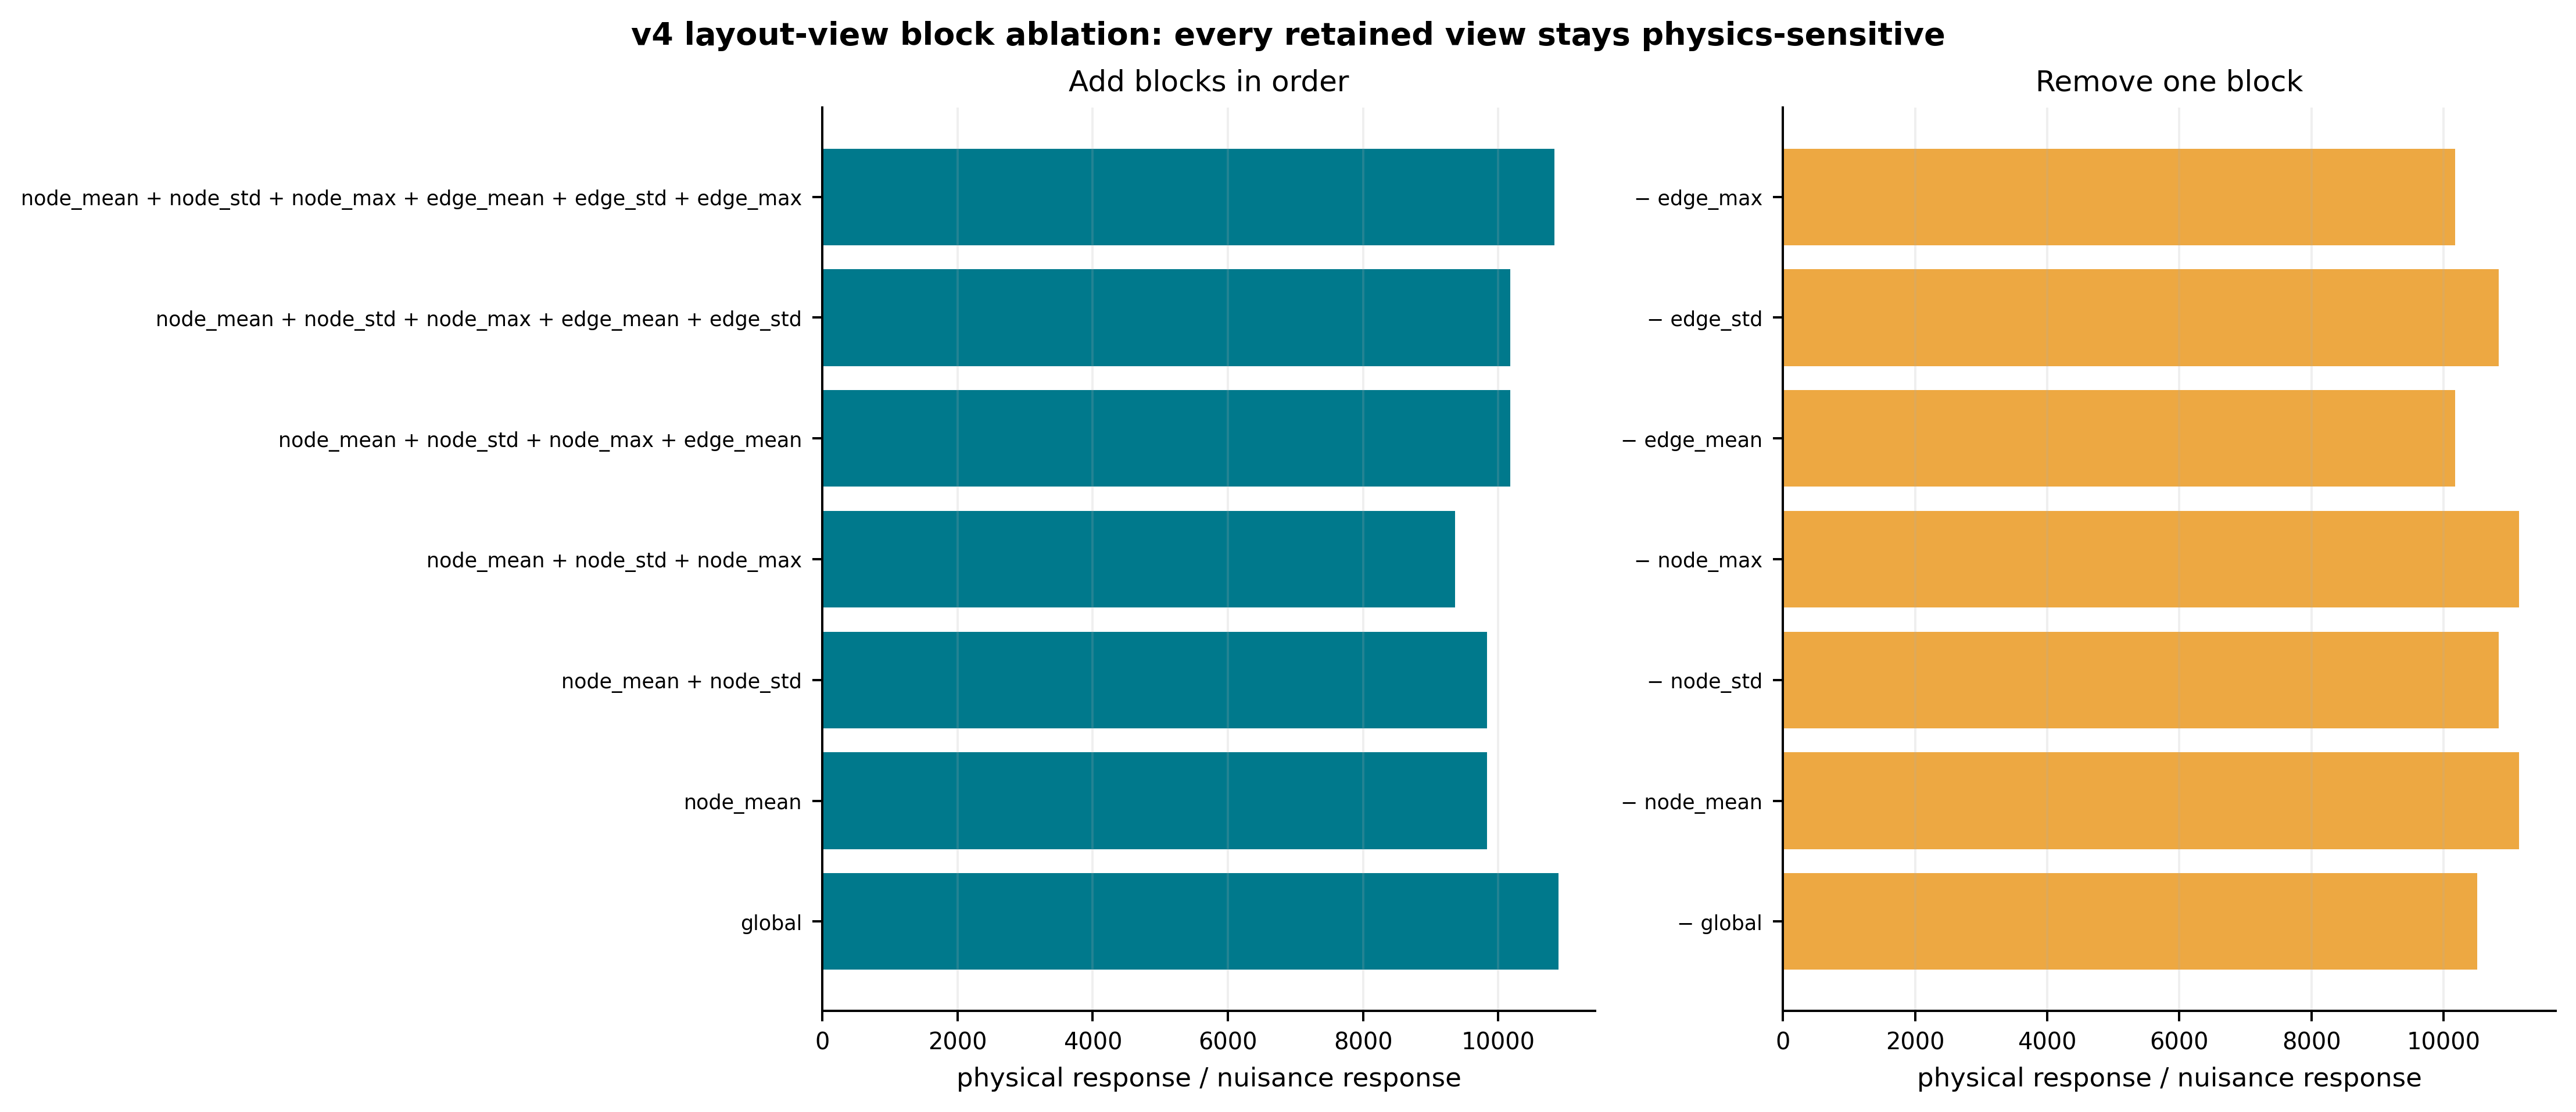
\includegraphics[width=\linewidth]{figures/generated/block_ablation.png}%
}{\missingfigure{block_ablation.png}}
\caption{Cumulative and drop-one-block ablation of v2 and later planar
representations. Each block is evaluated against both nuisance controls and
physical perturbations; downstream accuracy alone is not an acceptance test.
Every cumulative and drop-one v4 layout view retained a physical-to-nuisance
response ratio above $9.4\times10^3$.}
\label{fig:block-ablation}
\end{figure}

\subsection*{A component atlas tests breadth and structured sampling}
We instantiate and export one valid planar GDS for every feasible Qiskit Metal
component. Every attempted component remains in the audit table: unsupported,
invalid, or semantically ambiguous exports are exclusions to explain rather than
points to hide. We test uniqueness in the full representation and use a
two-dimensional projection only for visualization; separation in a projection
is not evidence of vector uniqueness.

Dense \texttt{GeneralizedCapNInterdigital} sweeps provide the principal
within-family example. The newly supplied sweep families and relevant
\squadds{} components test whether families occupy organized neighborhoods and
whether parameter sweeps trace reproducible trajectories through those
neighborhoods.

The frozen Qiskit Metal inventory contained 38 production classes. Thirty-six
could be exported as valid standardized planar GDS, while
\texttt{OpenToGround} and \texttt{ShortToGround} were retained in the manifest
as semantic/context-only entries rather than manufactured geometries. The 36
valid exports formed 31 independently measured physical-geometry equivalence
classes, and the v4 layout view produced exactly 31 vectors. Thus every observed
vector equality was explained by identical physical geometry. In a separate
deterministic sample of 144 supplied layouts (24 from each of six campaigns),
all 144 v4 layout vectors were distinct.

The exact-vector audit therefore found no unexplained collision in either the
Qiskit Metal singleton inventory or the sampled supplied campaigns. The
two-dimensional atlas is retained only as an interpretable visualization of
family structure; it is not used to certify uniqueness.

\begin{figure}[t]
\centering
\IfFileExists{figures/generated/qmetal_atlas.png}{%
  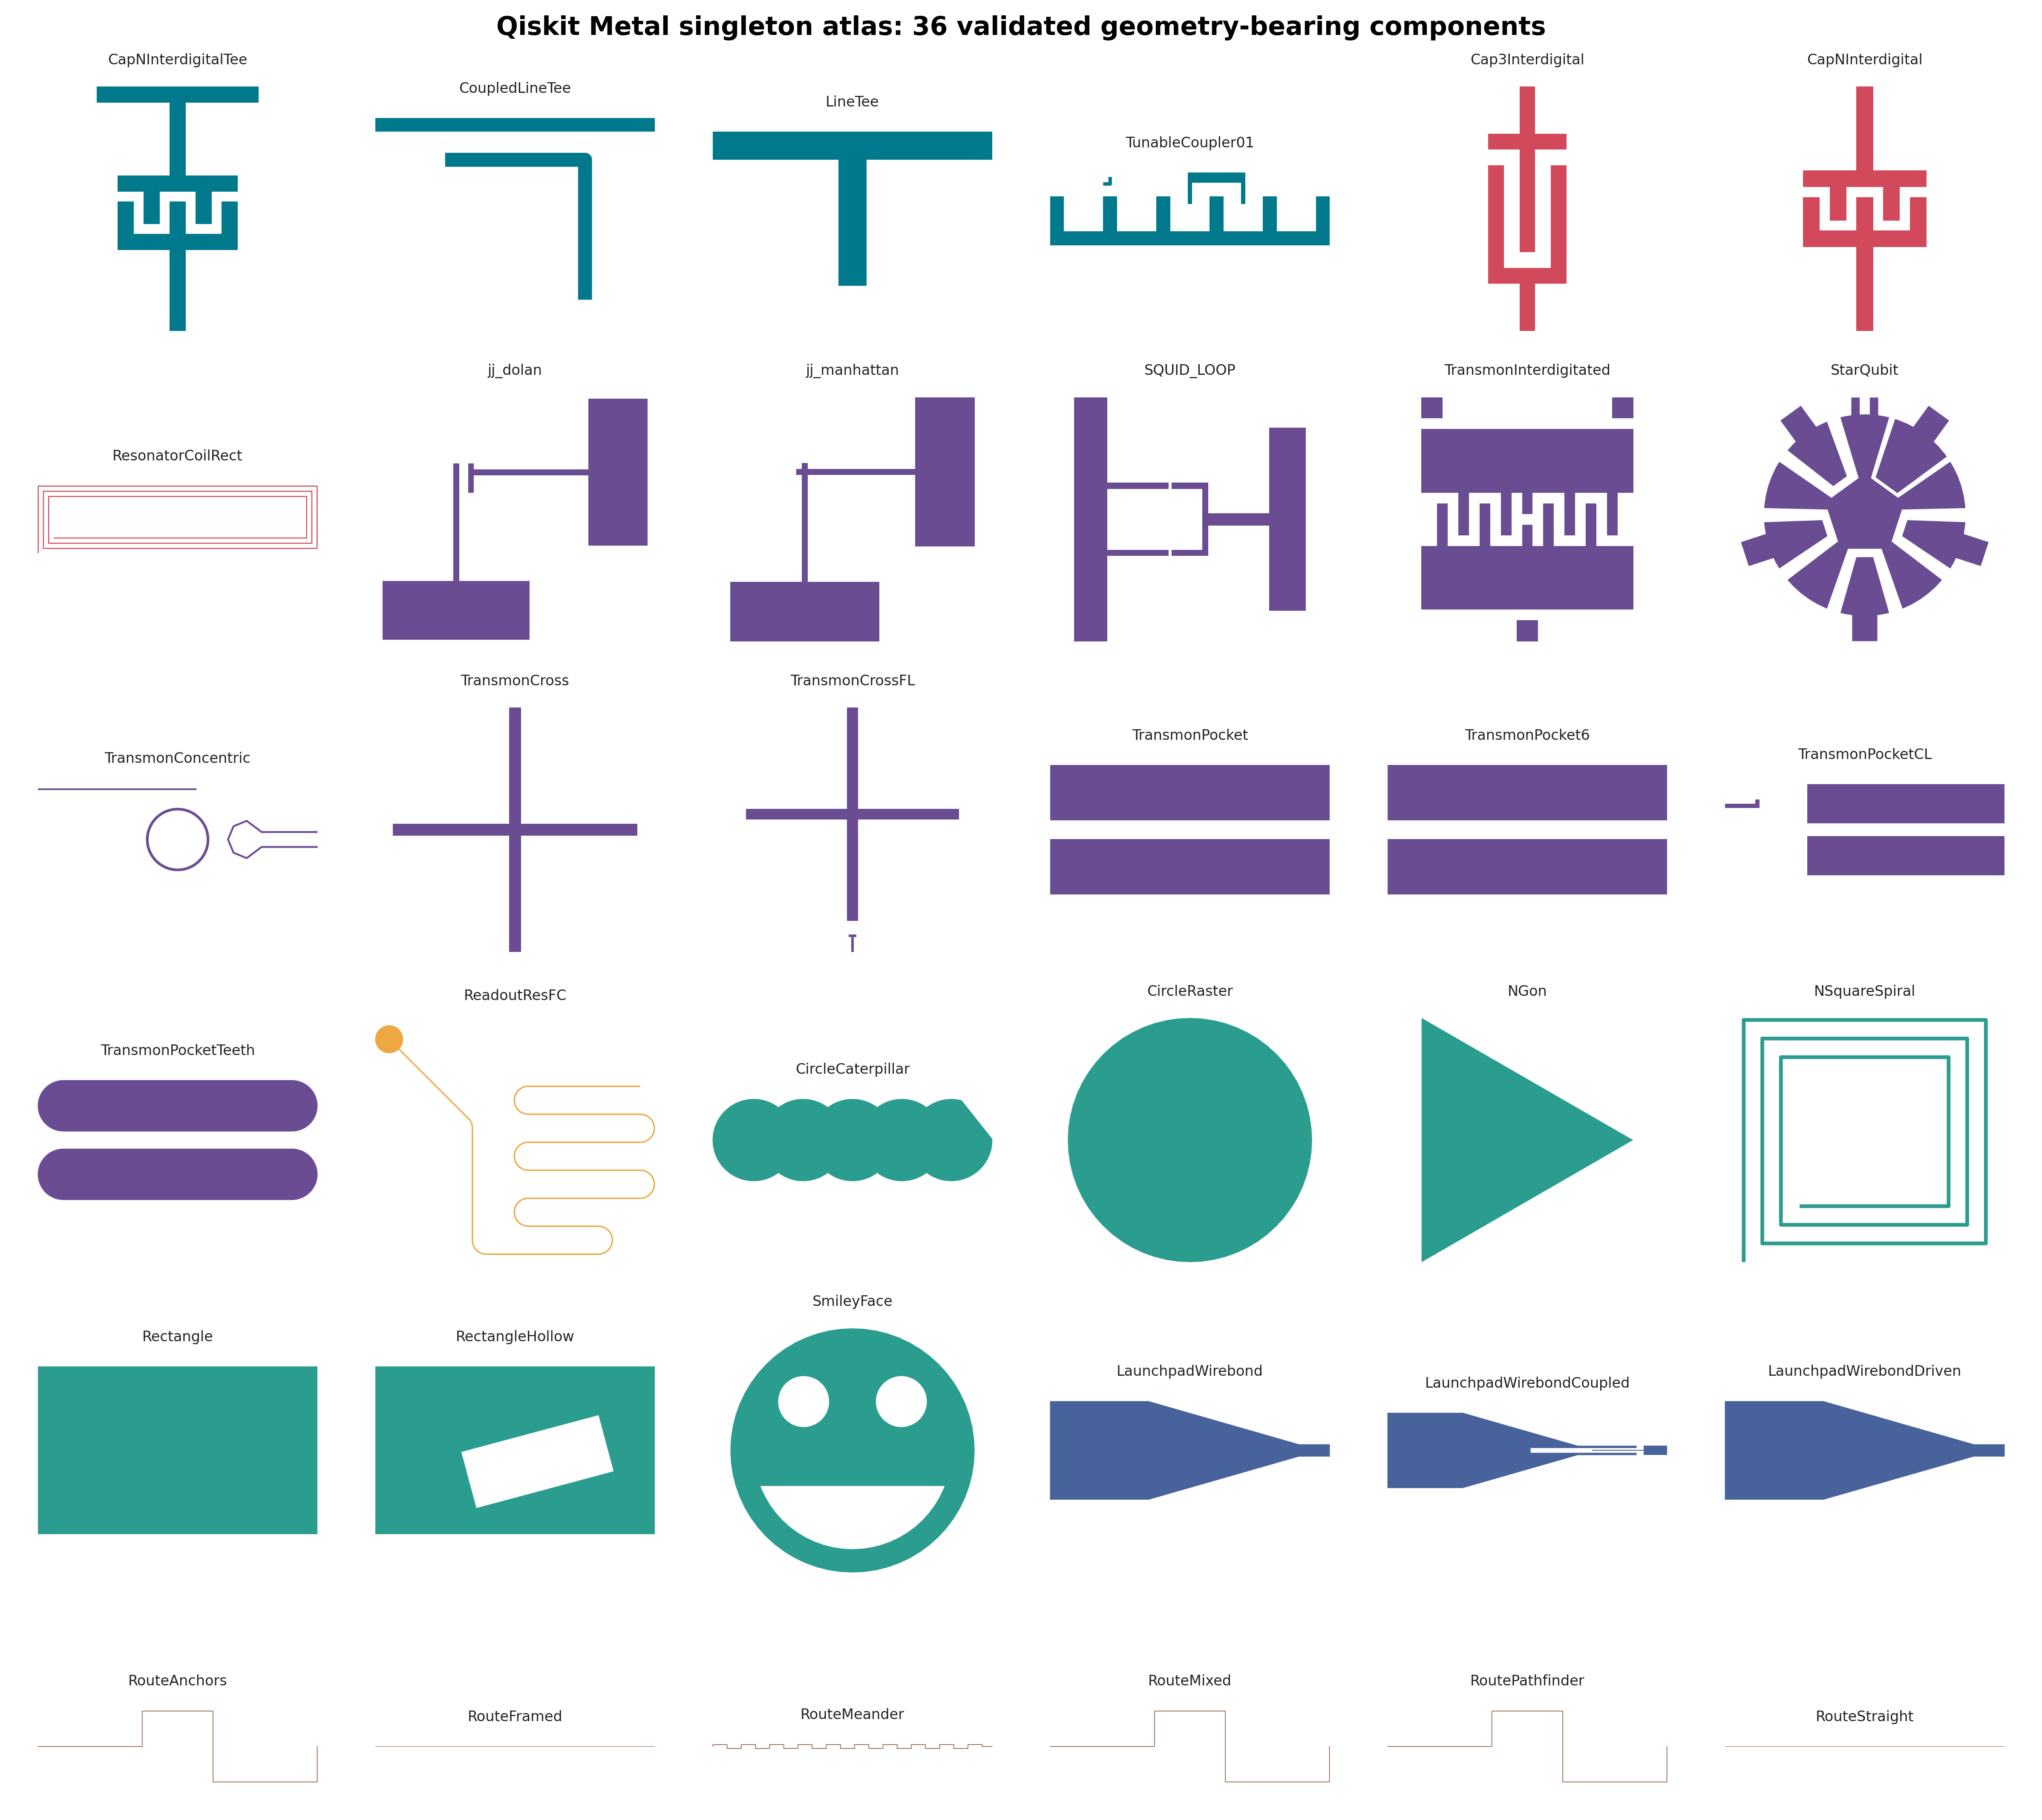
\includegraphics[width=\linewidth]{figures/generated/qmetal_atlas.png}%
}{\missingfigure{qmetal_atlas.png}}
\caption{Qiskit Metal singleton atlas and structured sweep coverage. Of 38
production classes, 36 yielded standardized planar GDS; these represented 31
physical-geometry equivalence classes and exactly 31 v4 layout vectors. The
two semantic/context-only classes remain in the audit manifest. A separate
supplied-layout sample contained 144 distinct vectors among 144 layouts; that
full-vector collision audit is reported in the text rather than inferred from
this two-dimensional atlas.}
\label{fig:qmetal-atlas}
\end{figure}

\subsection*{Planar composition preserves ports and galvanic topology}
The recordings motivate both representation differences and modular
composition. We therefore test differences along controlled parameter paths and
compare a port-aware composition of module representations with the embedding
computed directly from the joined GDS. Composition is not assumed to be raw
vector addition: relative position, scale, ports, shared ground, and conductor
merges must be supplied to the operation. A decisive example joins two
two-conductor modules so that one galvanic merge produces a three-conductor
system and a correspondingly different capacitance-matrix shape. Higher terminal
counts test that the interface is not specialized to this example.

Naive addition of the two 544-coordinate layout views had high cosine similarity
(0.991) but a relative error of 0.869 against the independently encoded joined
GDS, decisively rejecting raw addition as a composition law. Merging the shared
port/net in geometry space produced the correct three-conductor graph and a
$4\times4$ conductor-plus-ground proxy. Pose-matched physical difference
vectors agreed with cosine 0.99997 and relative error 0.0091; the wider-gap
control's $37^\circ$ rotation drift was $9.87\times10^{-4}$.

\begin{figure}[t]
\centering
\IfFileExists{figures/generated/modular_arithmetic.png}{%
  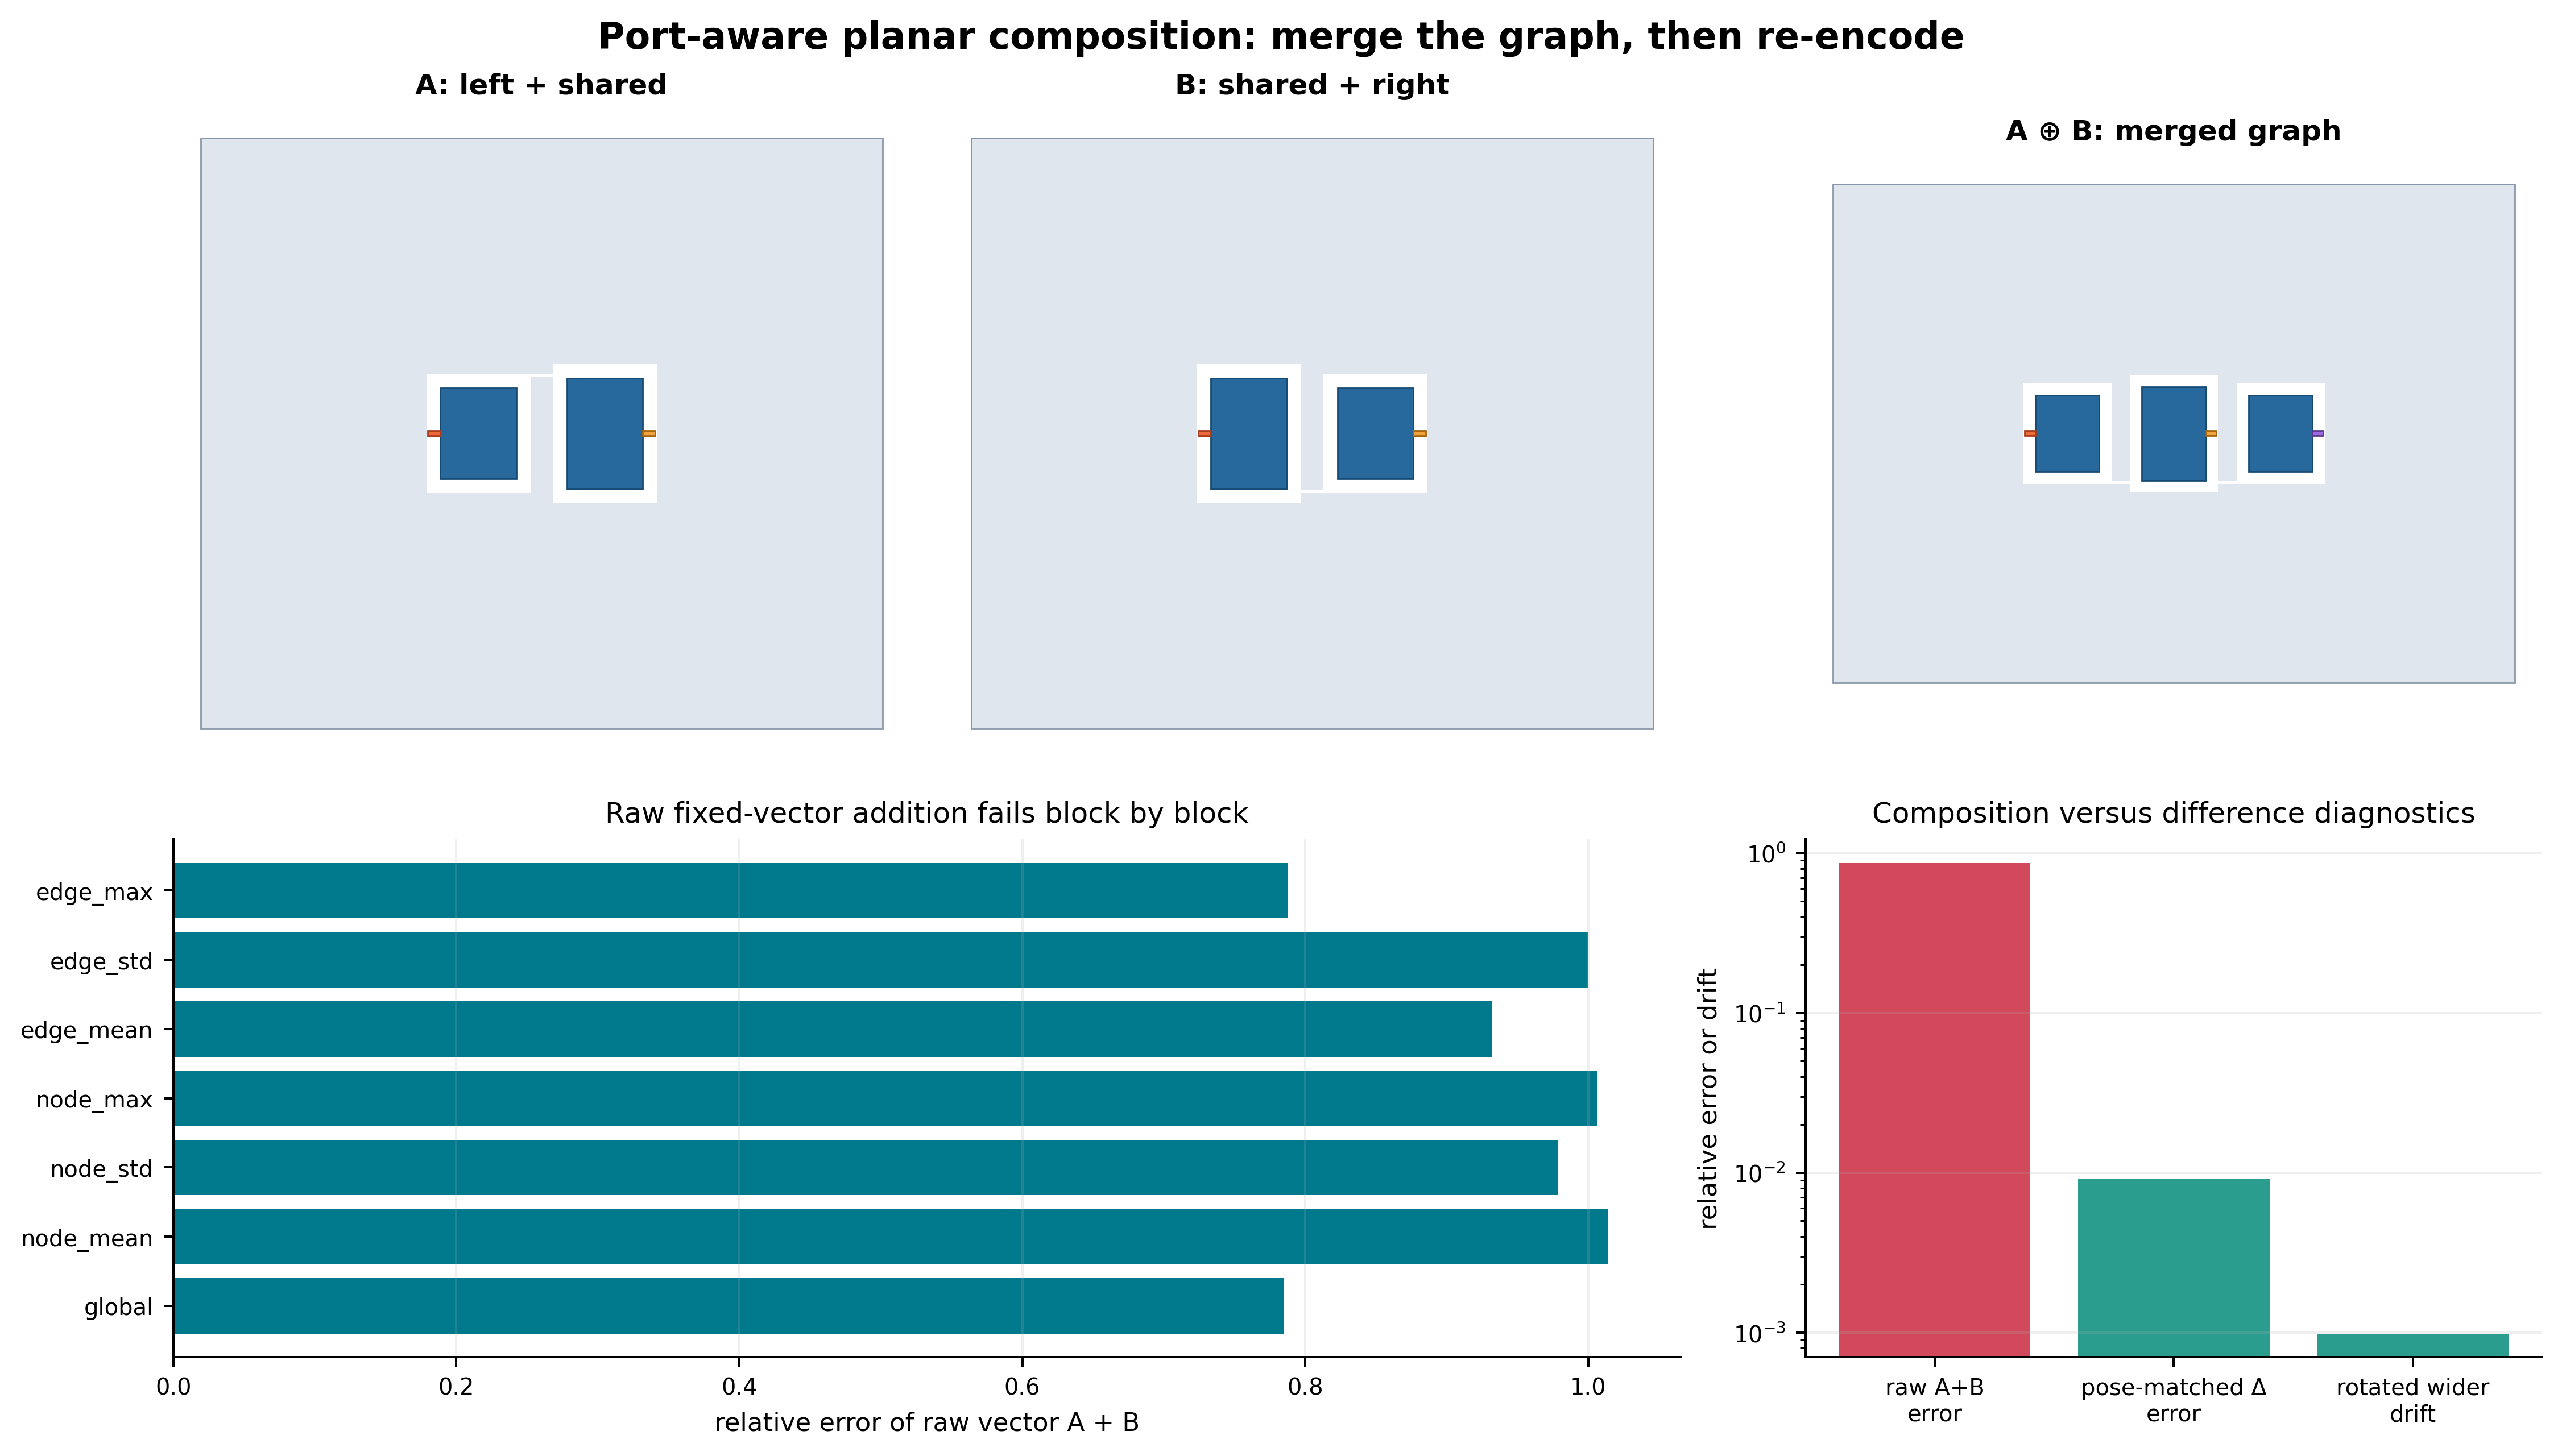
\includegraphics[width=\linewidth]{figures/generated/modular_arithmetic.png}%
}{\missingfigure{modular_arithmetic.png}}
\caption{Controlled representation differences and port-aware planar
composition. The required comparison is between a composed representation and
the independently parsed joined GDS, including conductor-graph and matrix-shape
agreement. Raw vector addition fails with 0.869 relative error, whereas graph
composition returns three conductors plus ground and pose-matched difference
directions agree to cosine 0.99997.}
\label{fig:modular-arithmetic}
\end{figure}

\subsection*{A common representation is compared with native parameter tables}
Embedding and native CSV/parameter-dictionary predictors receive identical
simulation labels, train/test identities, preprocessing budgets, and comparable
model capacity. We report in-family performance and then hold out entire
families. Because native schemas differ, their inability to form a common input
is documented explicitly rather than concealed by an arbitrary hand-aligned
table.

On repeated design-disjoint within-family splits, v4 reached mean $R^2$ values
of 0.987, 0.986, and 0.978 for generalized IDC, Tee, and transverse-cross
families. Native options reached 0.969, 0.940, and 0.981, respectively. Thus the
universal geometry view retained or improved within-family performance for the
two capacitors, whereas the compact native Transmon coordinates remained
slightly stronger for the cross and had lower absolute error.

As a provisional downstream audit using one frozen random-feature ridge head
and strict leave-one-family-out splits (894 designs per family), v4 obtained
$R^2$ values of 0.970, 0.743, and 0.727 for held-out
\texttt{CapNInterdigitalTee}, \texttt{GeneralizedCapNInterdigital}, and
\texttt{TransmonCross}, respectively. The corresponding RMSE values were
3.107, 1.002, and 1.331~fF, and median absolute errors were 1.060, 0.635, and
0.787~fF. v2 collapsed on the held-out transverse cross ($R^2=-2.494$;
RMSE 6.739~fF; median absolute error 5.119~fF). The v3 core remained slightly
better than v4 on that target ($R^2=0.792$), so repeated-seed and model-class
controls are still required before claiming v4 dominance.

\begin{figure}[t]
\centering
\IfFileExists{figures/generated/native_vs_embedding.png}{%
  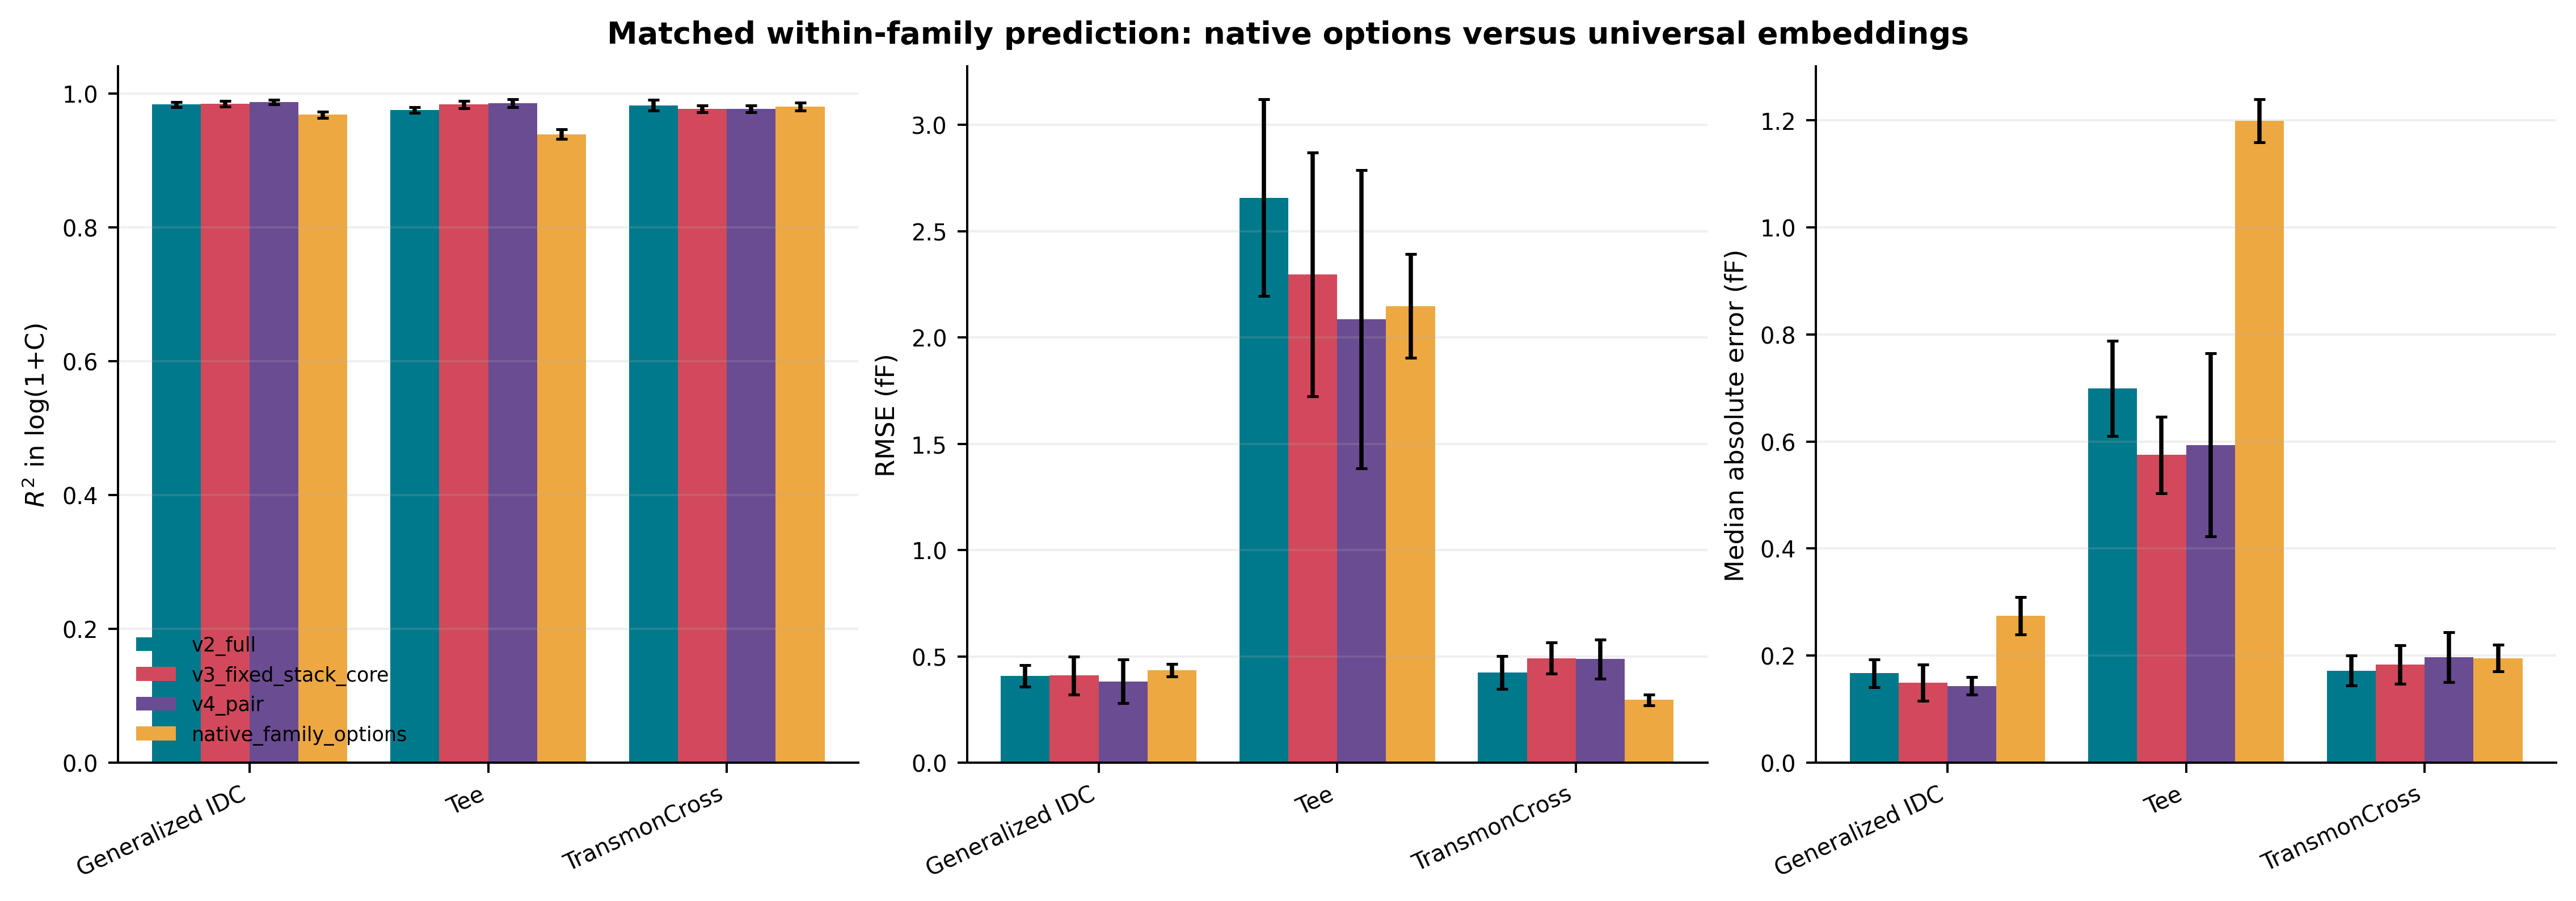
\includegraphics[width=\linewidth]{figures/generated/native_vs_embedding.png}%
}{\missingfigure{native_vs_embedding.png}}
\caption{Matched within-family native-parameter and embedding prediction.
Panels show repeated-split $R^2$, RMSE, and median absolute error under one
shared model protocol. v4 obtained $R^2=0.987$, 0.986, and 0.978; native
options obtained 0.969, 0.940, and 0.981. The separate leave-one-family-out
audit is reported in the text and does not establish v4 dominance on the
transverse-cross target.}
\label{fig:native-vs-embedding}
\end{figure}

\subsection*{Representation proximity is calibrated against capacitance}
We first compute a family-balanced similarity matrix and predeclare how unequal
family sizes are weighted. The nearest and most distant family pairs define two
transfer case studies. Across the full evaluation set, representation distance
is compared with normalized capacitance difference using design-cluster
uncertainty intervals. Similarity is treated as a hypothesis about transfer,
not a physical result by itself.

Across 12,000 family-balanced design pairs, Spearman association between
embedding distance and normalized capacitance difference was 0.082 for v2,
0.255 for the v3 fixed-stack core, and 0.251 for the v4 pair view. Design-cluster
bootstrap 95\% intervals were [0.073, 0.123], [0.237, 0.296], and [0.235,
0.294], respectively. The positive but modest values support geometry distance
as a retrieval prior, not as a calibrated capacitance metric.

\begin{figure}[t]
\centering
\IfFileExists{figures/generated/similarity_capacitance.png}{%
  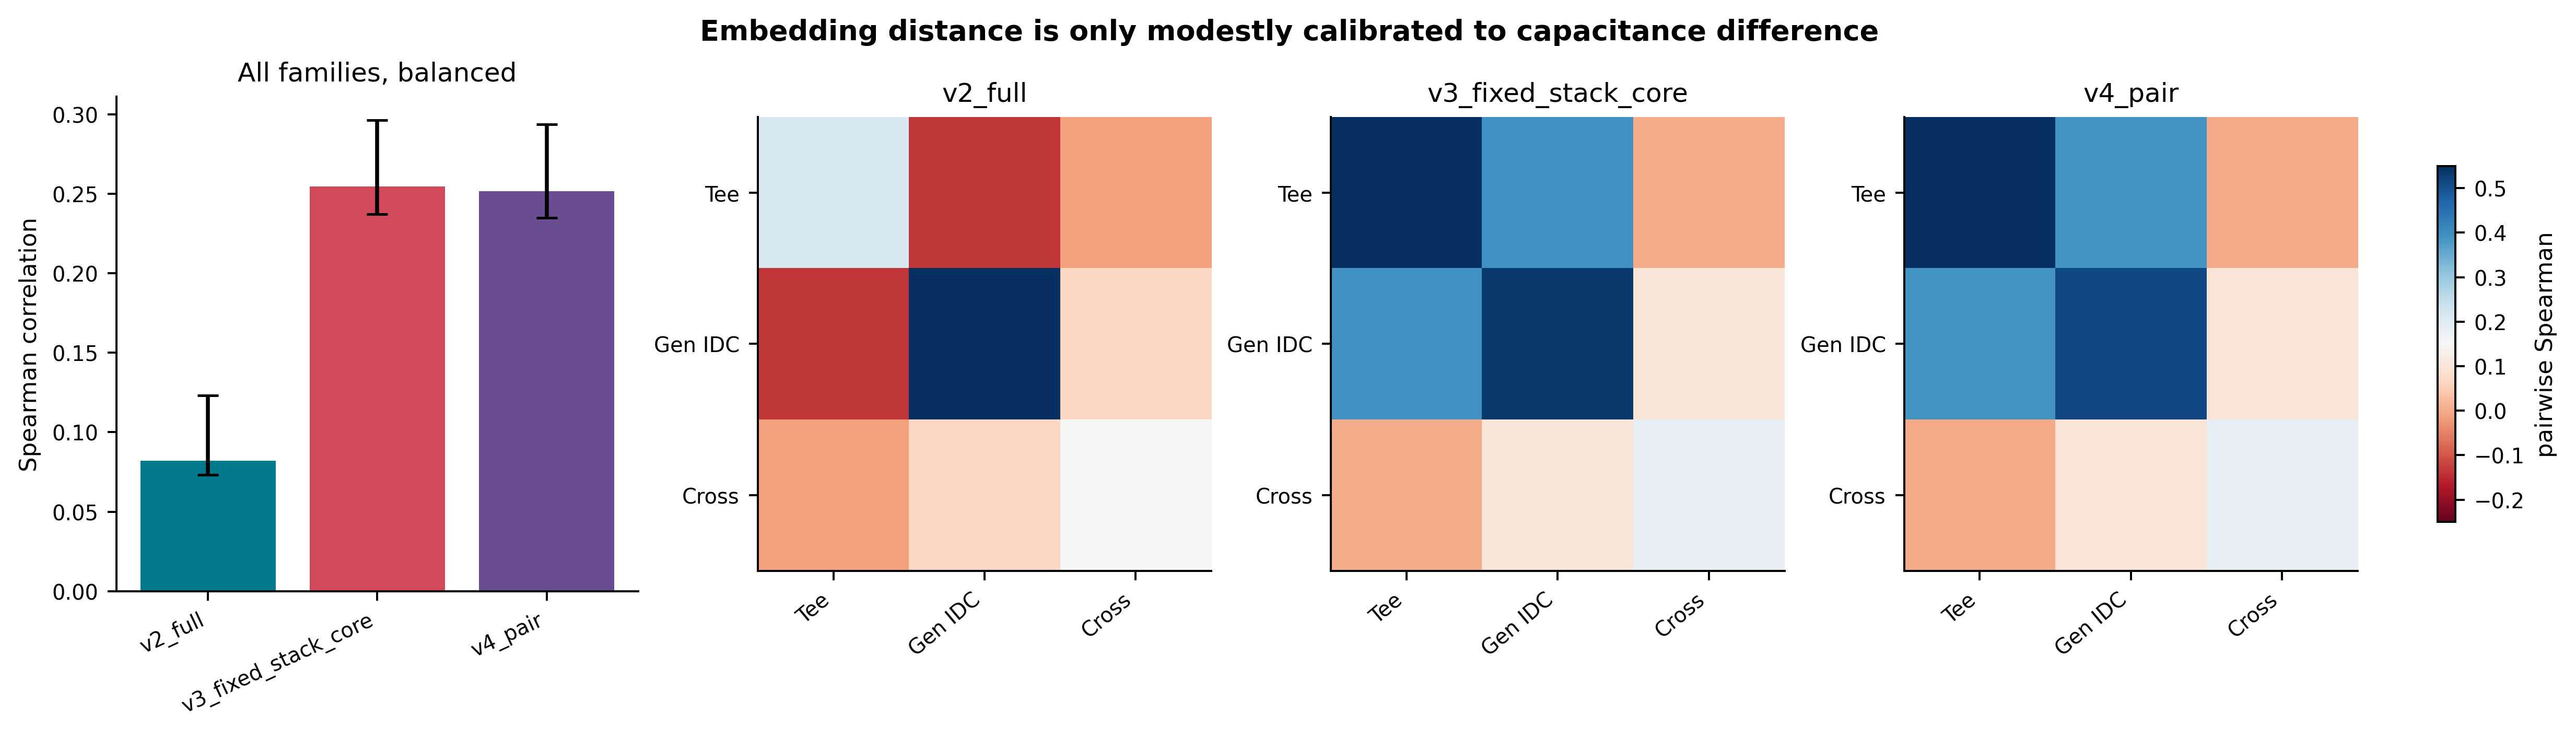
\includegraphics[width=\linewidth]{figures/generated/similarity_capacitance.png}%
}{\missingfigure{similarity_capacitance.png}}
\caption{Representation proximity versus capacitance difference. The left
panel reports the family-balanced association with design-cluster bootstrap
intervals; the remaining panels expose within- and cross-family variation for
each representation. The balanced v4 association is
$\rho=0.251$ with 95\% interval [0.235, 0.294], comparable with v3 and stronger
than v2, but far from a one-to-one capacitance metric.}
\label{fig:similarity-capacitance}
\end{figure}

\subsection*{Near- and far-family transfer is measured by target-label efficiency}
For both the high-similarity and low-similarity source--target family pairs, a
source specialist is adapted using nested target subsets of 1, 5, 10, 50, and
100 simulations. The target test set remains fixed. Source-initialized models
are compared with target-only and no-transfer baselines over repeated seeds.
The primary endpoint is the number of target simulations needed to reach a
predeclared matrix-error tolerance; conventional $R^2$, RMSE, and MAE are
secondary summaries.

The repeated learning curves did not show a universal source-transfer
advantage. At 100 target labels, target-only v4 achieved mean $R^2=0.943$, RMSE
1.936~fF, and median absolute error 0.584~fF, compared with $R^2=0.911$,
RMSE 2.408~fF, and median absolute error 0.765~fF for pooled source-plus-target
training. One-label estimates were unstable and negative in mean $R^2$ for all
methods. Near/far geometry-centroid selection therefore did not overcome the
solver-campaign and topology confounding in these historical tables.

\begin{figure}[t]
\centering
\IfFileExists{figures/generated/transfer_learning.png}{%
  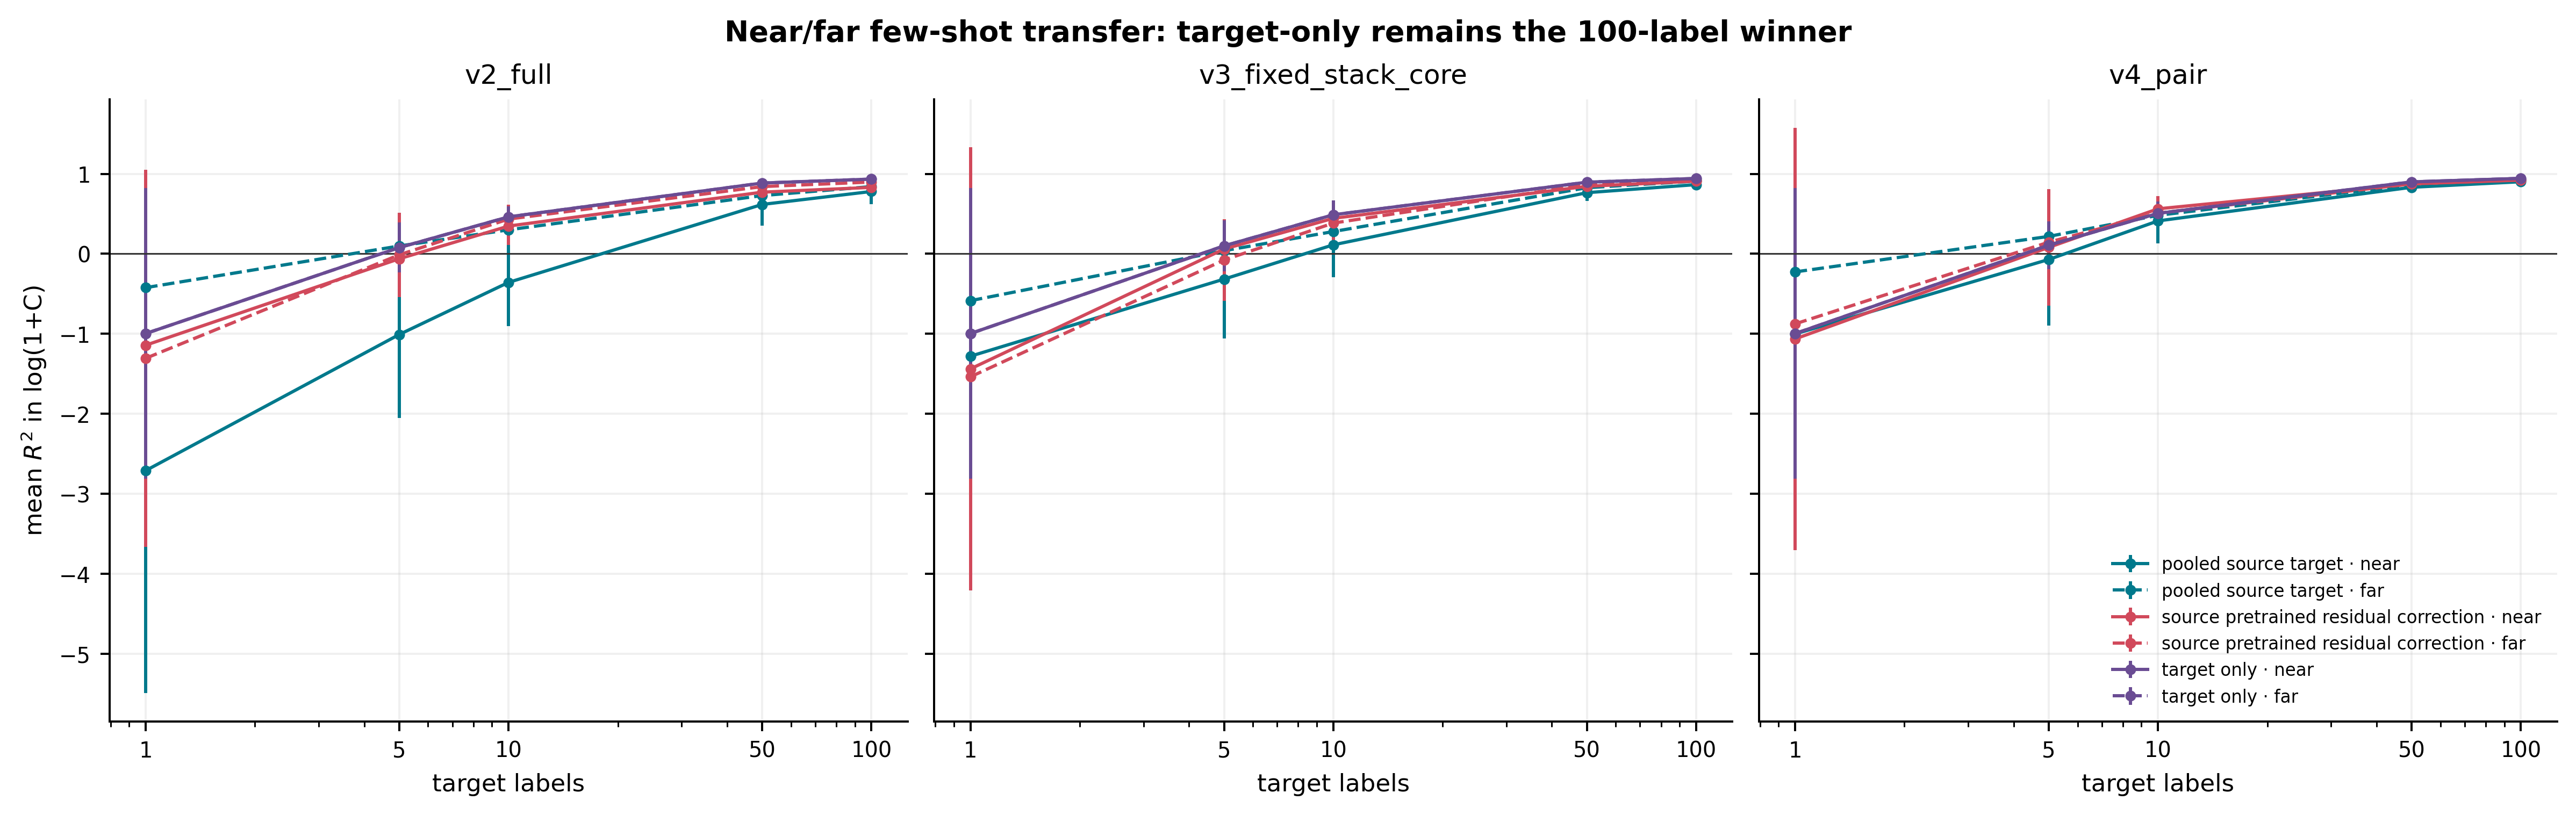
\includegraphics[width=\linewidth]{figures/generated/transfer_learning.png}%
}{\missingfigure{transfer_learning.png}}
\caption{Target-label efficiency for near- and far-family transfer. Curves use
the same fixed target test set and nested target subsets of 1, 5, 10, 50, and
100 simulations, with target-only, pooled, and residual-correction controls.
At 100 labels the target-only v4 curve is the strongest of the tested v4
methods; the present cohort therefore supplies a negative control rather than
a universal transfer-win claim.}
\label{fig:transfer-learning}
\end{figure}

\subsection*{Controlled diversity tests a generalist model}
Generalist training sets grow in a controlled sequence: more samples within a
family, nearby families, distant families, and mixtures that expand coverage of
representation space. Sample-count-matched controls separate diversity from
dataset size. Every model is evaluated on the same validation sets, including a
family absent from training. Leave-one-cluster-out, within-cluster
interpolation, nearby extrapolation, cluster-edge, and heavy-tail analyses test
whether the model learned local structure or collapsed toward a global mean.

Matched-budget family diversity was consistently more useful than adding rows
from only one topology. With 600 training designs drawn from all three families,
mean cross-task $R^2$ was 0.881 for v2, 0.942 for v3, and 0.941 for v4. In
contrast, 600 designs from one family gave mean $R^2$ values of $-1.091$,
$-0.601$, and $-0.356$, respectively, because unseen-family predictions
remained poor.

\begin{figure}[t]
\centering
\IfFileExists{figures/generated/generalist_growth.png}{%
  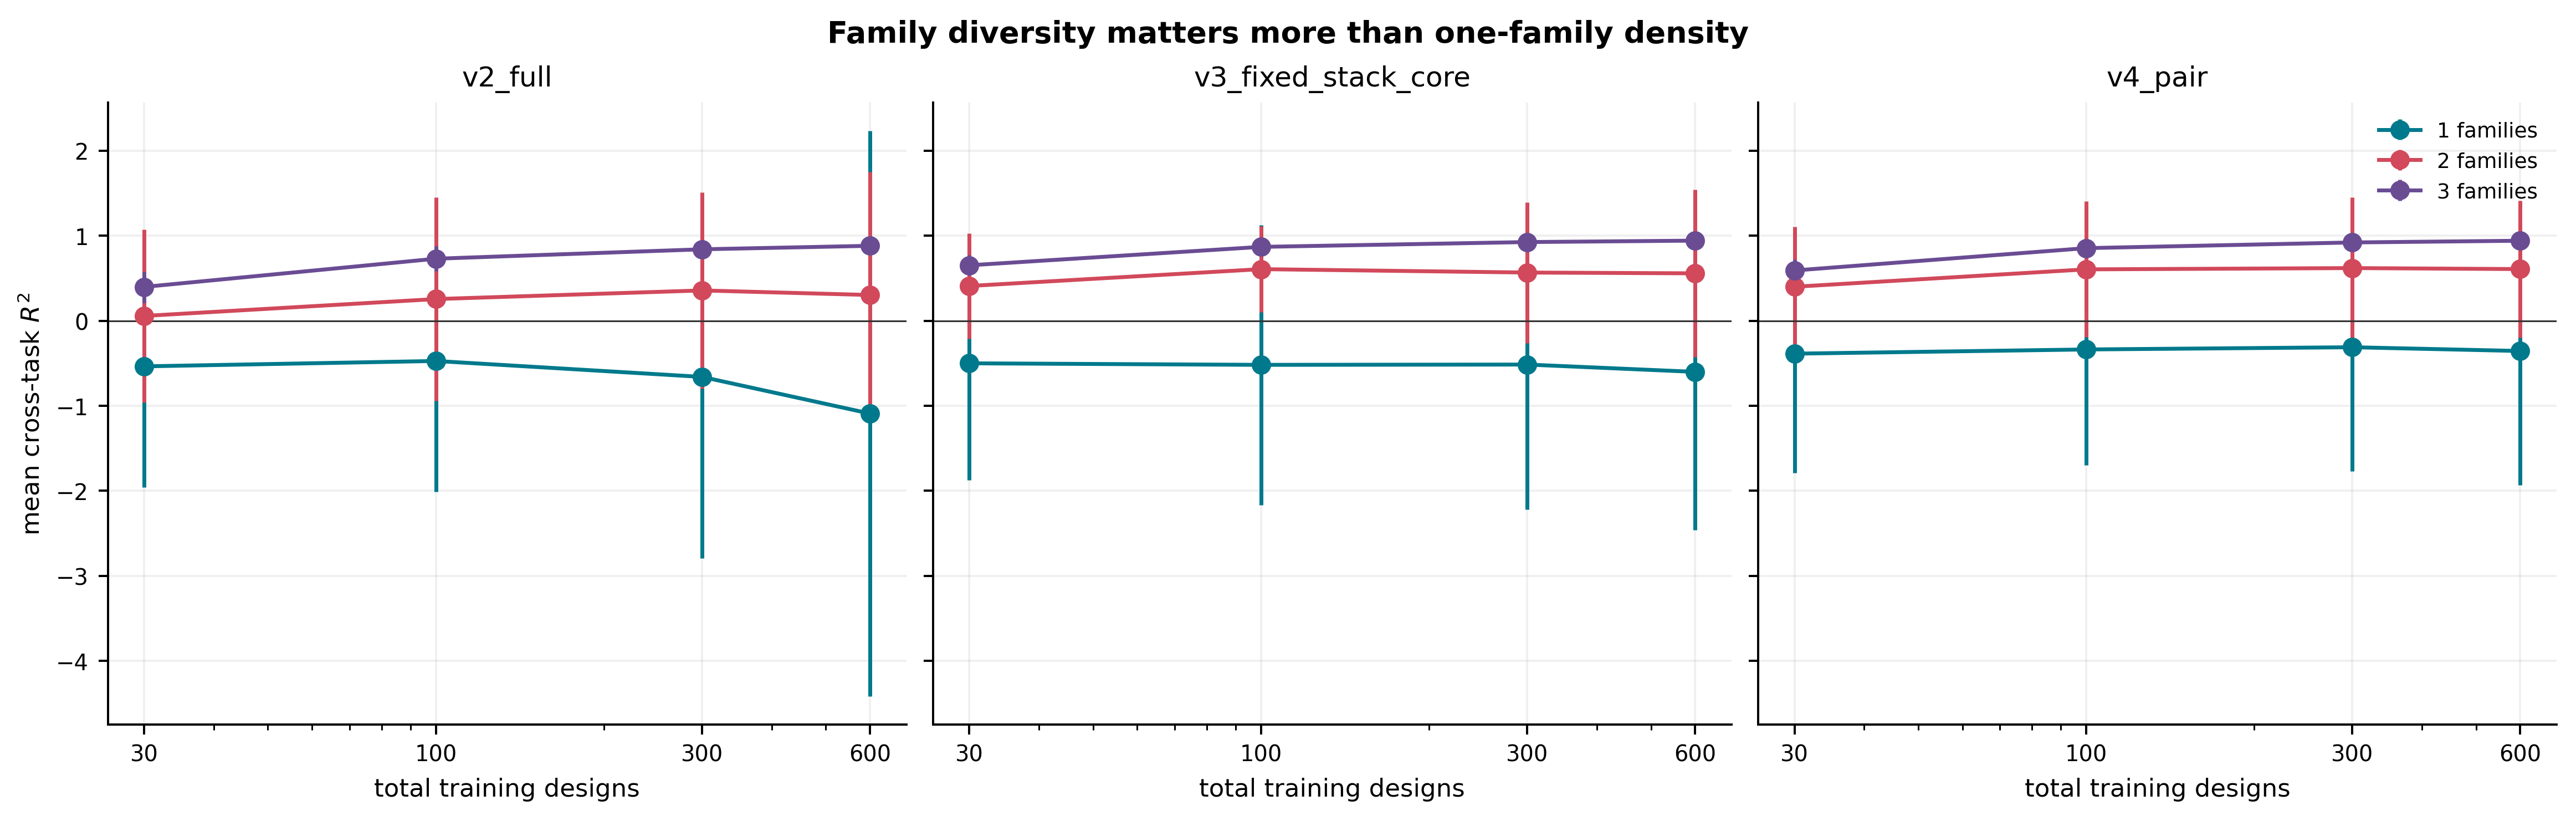
\includegraphics[width=\linewidth]{figures/generated/generalist_growth.png}%
}{\missingfigure{generalist_growth.png}}
\caption{Controlled growth of a planar generalist model. Sample-count-matched
stages separate within-family density from nearby-family, distant-family, and
mixed-family diversity. At 600 designs, three-family v3/v4 training reaches
mean cross-task $R^2\approx0.94$, whereas one-family training remains negative;
topology coverage, not row count alone, controls generalization.}
\label{fig:generalist-growth}
\end{figure}

\subsection*{An unseen composite system closes the workflow}
The final structural experiment connects previously modeled planar modules into
a multi-terminal component absent from training. Before any predictive claim,
the pipeline must identify the new conductor graph and requested
capacitance-matrix shape. A subsequent high-fidelity composite sweep and
target-only adaptation control are intentionally deferred until converged
solver labels exist.

The unseen joined GDS was parsed as three signal conductors with no unmarked
island and produced the expected $4\times4$ symmetric conductor-plus-ground
low-fidelity operator. This is a structural zero-shot pass only. Because no
converged three-dimensional capacitance matrix or composite sweep is currently
available, zero-shot accuracy and adaptation curves are explicitly untested.

\begin{figure}[t]
\centering
\IfFileExists{figures/generated/unseen_composite.png}{%
  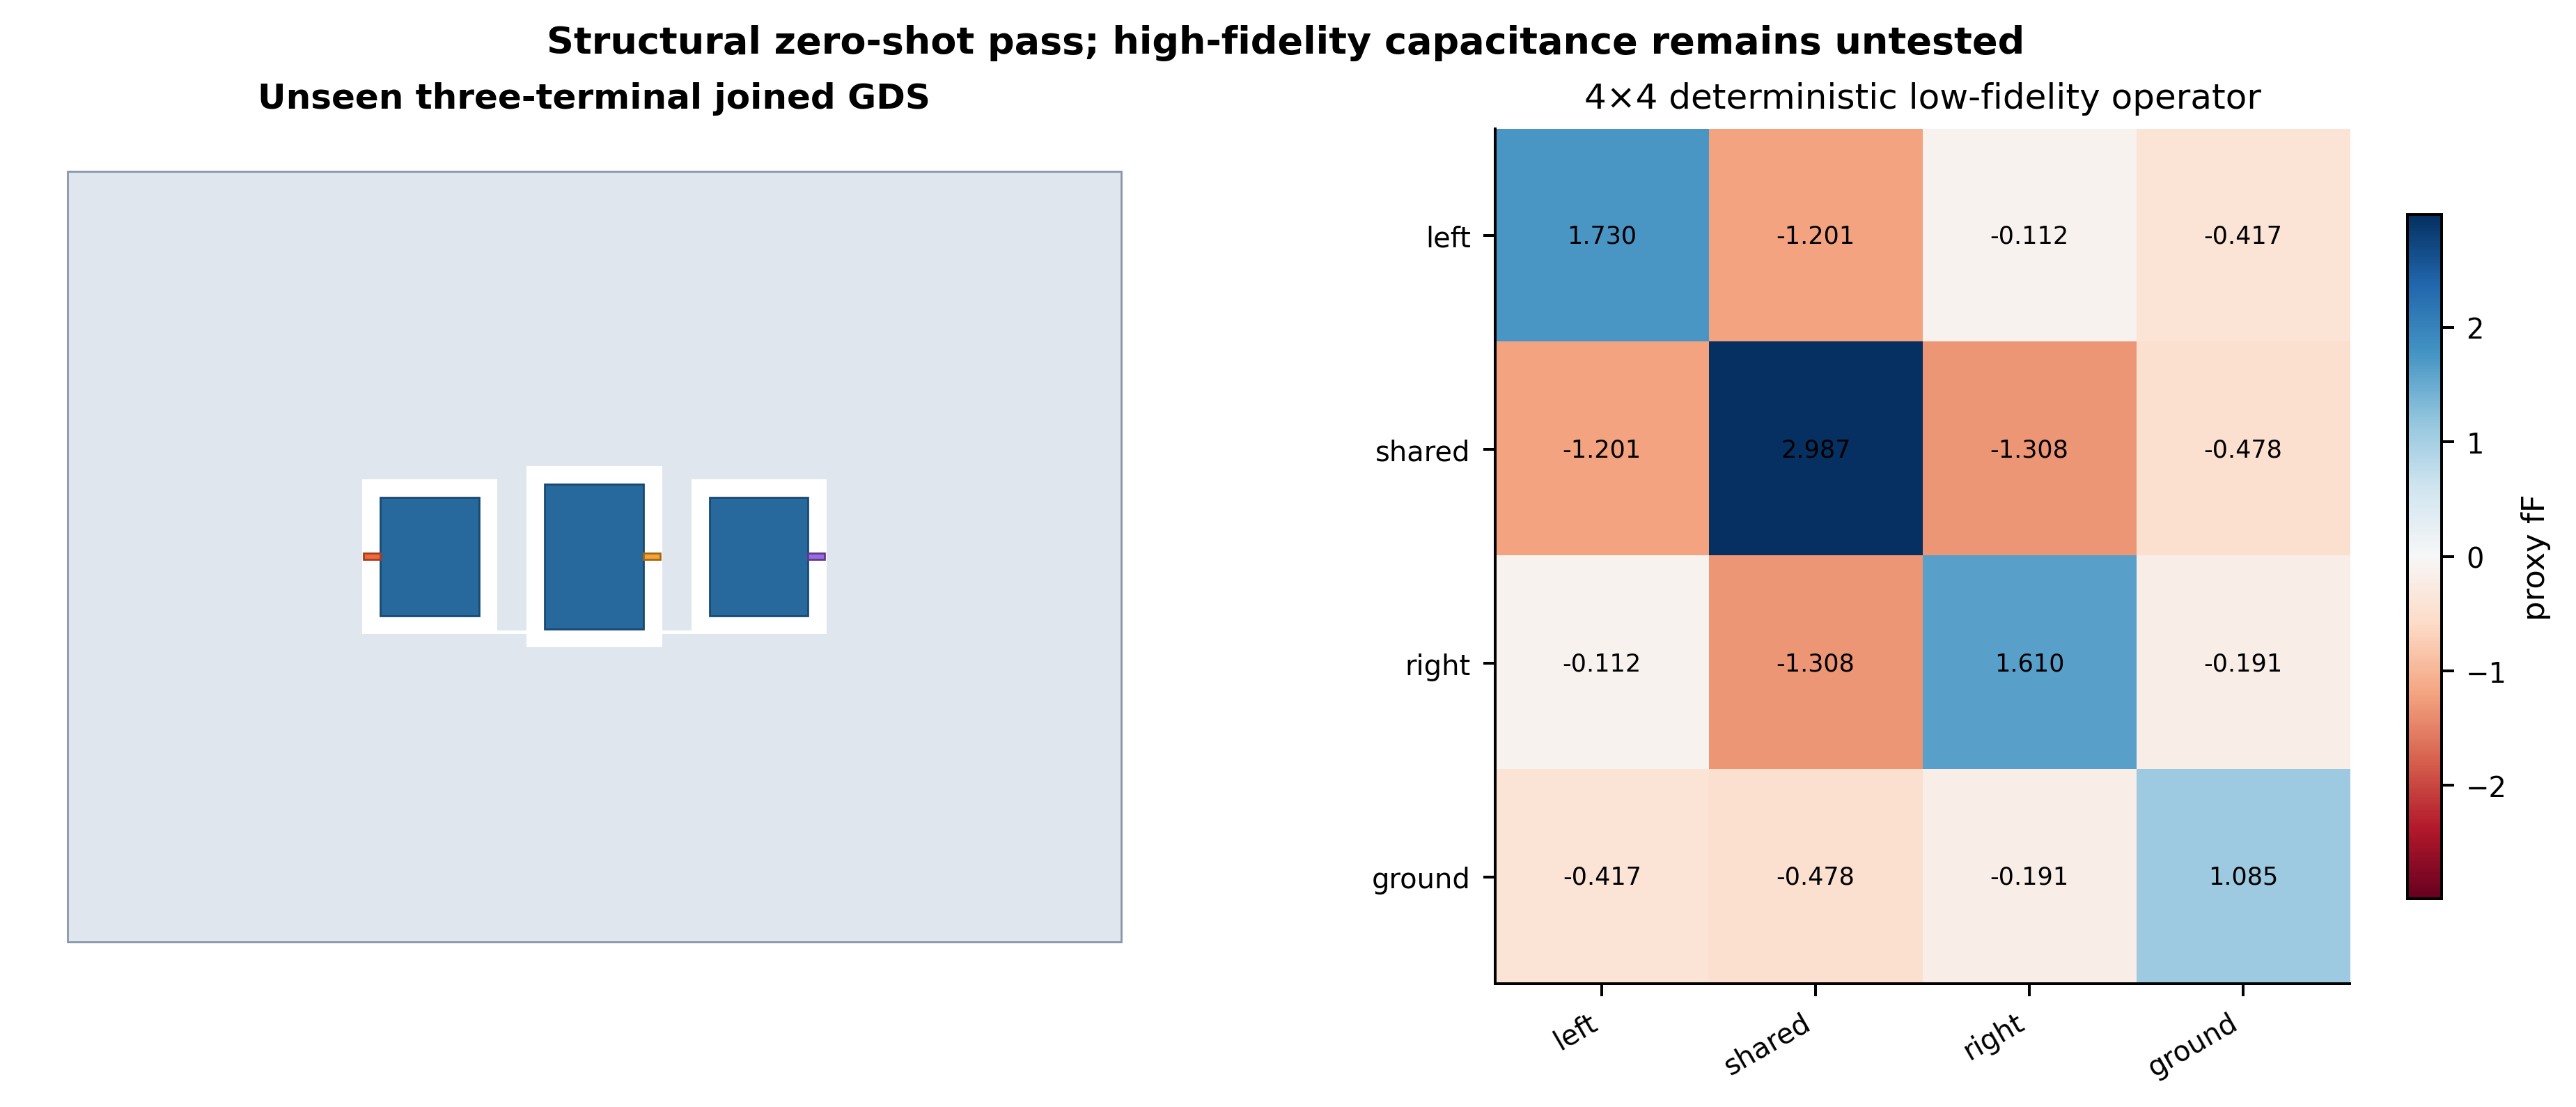
\includegraphics[width=\linewidth]{figures/generated/unseen_composite.png}%
}{\missingfigure{unseen_composite.png}}
\caption{Unseen planar composite structural test. The standardized GDS is
parsed as three signal conductors, and v4 emits the corresponding $4\times4$
low-fidelity conductor-plus-ground operator. This is not a high-fidelity
zero-shot prediction; composite solver labels and a target-only adaptation
control remain identified data-acquisition requirements.}
\label{fig:unseen-composite}
\end{figure}

\section*{Discussion}
The intended contribution is an auditable bridge between otherwise incompatible
simulation datasets, not a claim that a learned surrogate replaces
electromagnetic simulation. The representation tests establish whether its
coordinates behave physically; held-out-family and composite experiments then
measure whether that prior reduces the need for new high-fidelity labels.

The current validation scope is planar. The software interface should reserve a
versioned JSON or XML mapping from GDS layer/datatype to plane, material,
thickness, and dielectric environment. Flip-chip claims require crossed
geometry--stack sweeps, same-projection/different-plane controls, and held-out
stack tests, and are deferred until those data exist. Likewise, ``foundation
model,'' universal composition, and transfer to semiconductor or photonic
devices remain future claims unless directly demonstrated.

\section*{Methods}

\subsection*{Planar GDS semantics and validation}
The exact layer/datatype assignments are versioned with the dataset rather than
hard-coded in the scientific claim. The schema identifies signal and ground
regions, named or ordered terminals, exclusions/etch, and connectivity rules.
Before embedding, every file is checked for valid geometry, connected-component
structure, terminal attachment, and consistency between terminal/conductor
count and the requested capacitance matrix.

\subsection*{Representation acceptance metrics}
For vectors $e(x)$ and paired transformations $T$, relative drift is
\begin{equation}
  d_T = \frac{\lVert e(Tx)-e(x)\rVert_2}
  {\max(\lVert e(x)\rVert_2,\epsilon)}.
\end{equation}
Nuisance transformations are required to remain below frozen numerical
tolerances. Physical paths must be non-degenerate and locally smooth; monotonic
ordering is required only for features and controls for which the physical
direction is justified. We additionally report blockwise effects so aggregate
normalization cannot mask a failed block.

For arbitrary terminal sets, relabeling tests require the conductor/terminal
representation and predicted matrix to transform equivariantly under the same
permutation. Matrix errors are reported per independent entry and with a
predeclared matrix-level aggregation.

\subsection*{Predictive and transfer evaluation}
All preprocessing is fitted on training data only. Grouped splits use stable
design identities so duplicate geometry cannot cross train and test sets.
Held-out-family tests, nested target-data learning curves, and diversity
ablations use fixed test sets, repeated seeds, and uncertainty intervals.
Family-pair selection is based on training-side representation statistics,
without consulting held-out target labels.

\section*{Data and code availability}
Code, GDS generation recipes, semantic schemas, acceptance thresholds, executed
notebooks, and exact exclusion logs will be released with immutable versions
after review. No external repository or dataset hub is modified by this working
draft.

\bibliographystyle{unsrt}
\bibliography{references}
\end{document}
